\documentclass[11pt]{article}
\title{How the Codynamic Book Machine Works}
\author{Arthur Petron}
\usepackage[margin=1in]{geometry}
\usepackage{graphicx}
\usepackage{amsmath,amssymb,mathtools}
\usepackage{tikz}
\usetikzlibrary{positioning,arrows.meta}
\usepackage{hyperref}
\graphicspath{{media/}{media/diagrams/}{images/}{artwork/}}

\begin{document}

\section{Abstract}

% CBM-SECTION-START:abstract:Abstract

The Codynamic Book Machine is a schema-backed, message-coordinated, multi-agent authoring system for producing books as living technical objects. Rather than treating a manuscript as a static sequence of files, the system represents authorial intent, outline structure, section drafts, editorial maintenance, references, diagrams, and compiled artifacts as coordinated state surfaces that evolve together through explicit tasks and durable messages. This paper presents the machine as both a writing environment and a working case study in codynamic architecture: a system in which content, code, agents, logs, and outputs remain mutually inspectable and continuously revisable.

The central claim is that long-form technical writing becomes more reliable when the book is modeled as a canonical work object and decomposed into section-level responsibilities handled by specialized agents. In this design, a hypervisor orchestrates work, section agents draft and revise local prose, a gardener agent performs editorial maintenance, a references agent owns citation support, and a diagram agent manages visual assets. These agents do not mutate the manuscript invisibly; they operate through queued tasks, append-only messages, and registered artifacts, so that every substantive change is traceable and reviewable.

The paper focuses on the repository that implements this workflow and uses it as evidence for the architecture it describes. It explains how outline intake becomes normalized structure, how task queues and callbacks coordinate agent work, how citations and diagrams are routed through specialist handoffs, and how generated \LaTeX{} payloads are separated from imported source material. The contribution is therefore twofold: a concrete authoring system that can be inspected and extended, and a technical account of how books can be managed as durable, machine-readable, collaboratively maintained systems rather than as isolated text files.


% CBM-SECTION-END:abstract

\section{Introduction}

\subsection{The Coordination Problem in Long-Form Writing}

% CBM-SECTION-START:ch01_sec01_problem:The Coordination Problem in Long-Form Writing

Long-form writing fails for a simple reason: the work is not one thing. A book is an evolving collection of outlines, section drafts, claims, citations, figures, editorial notes, and build artifacts, each of which can change at a different pace. When those parts are managed separately, they drift. The outline may promise a structure that the prose no longer follows; a section may introduce a claim that never receives a citation; a diagram may reflect an earlier argument; a review comment may be resolved in one file but remain visible in another; and a successful build may conceal the fact that the manuscript is internally inconsistent.

This drift is especially costly in long-form technical writing, where coherence depends on more than local correctness. A chapter can read well sentence by sentence while still failing at the level of argument, terminology, or dependency order. A definition introduced in one section may be reused elsewhere before it is stabilized. A reference added late in the process may support one paragraph but not the surrounding discussion. A figure can become stale as soon as the surrounding explanation changes. Even the compiled output can lag behind the source of truth if the manuscript is assembled from multiple moving parts without a disciplined coordination model.

The problem is not merely that books are large. It is that they are heterogeneous. The outline expresses intent, the draft expresses prose, the bibliography expresses evidence, the diagram set expresses structure, the review cycle expresses editorial judgment, and the build system expresses what can actually be compiled. If these surfaces are treated as independent, authors and tools must continually reconstruct the relationships among them by hand. That reconstruction is fragile, repetitive, and easy to get wrong.

In conventional workflows, this fragility appears as familiar failure modes. An outline is revised after sections have already been drafted, leaving the manuscript misaligned with the plan. A citation is added in one place but not propagated to related claims. A diagram is requested too early and then forgotten when the argument changes. Review feedback is recorded in comments, but the corresponding text is not updated consistently across files. Build errors are fixed locally without addressing the underlying dependency that caused them. Over time, the manuscript accumulates small inconsistencies that are individually minor but collectively expensive.

The coordination problem, then, is the challenge of keeping all of these surfaces synchronized while the book is still being written. It is not enough to generate text; the system must preserve alignment among intent, structure, evidence, visuals, editorial state, and compiled artifacts. The Codynamic Book Machine is designed around that requirement. Its central claim is that a book can be managed as a living technical object only if the relationships among its parts are made explicit and continuously maintained.

That requirement motivates the rest of this paper. The next section states the thesis of the machine as a codynamic system: one in which outline, agents, task queues, dependencies, artifacts, and compiled outputs evolve together rather than as isolated files. Subsequent sections ground that thesis in the repository itself, showing how the current implementation represents the work, routes tasks, registers references, requests diagrams, and preserves a durable record of the manuscript as it changes.

\begin{figure}[htbp]
\centering
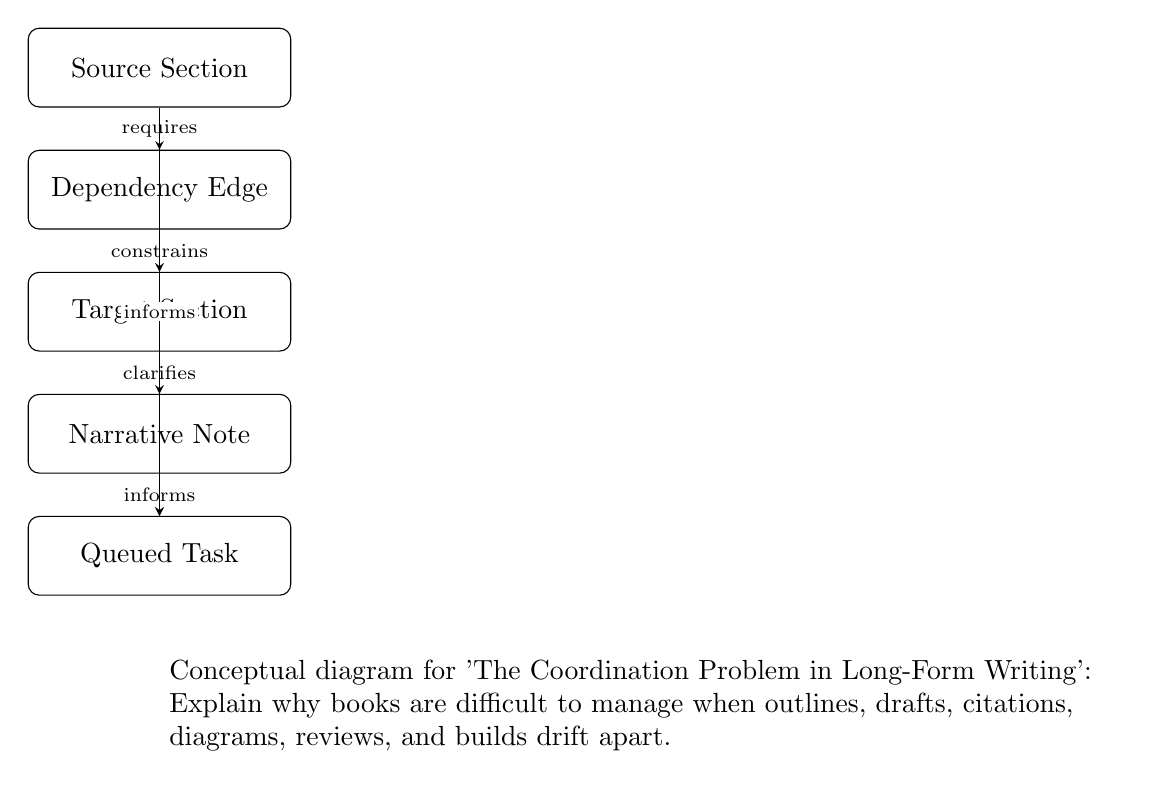
\begin{tikzpicture}[>=stealth, node distance=2.2cm,
  concept/.style={draw, rounded corners, align=center, text width=3.1cm, minimum height=1cm},
  relation/.style={font=\scriptsize, fill=white, inner sep=1pt}]
\node[concept] (n1) at (0,0.0) {Source Section};
\node[concept] (n2) at (0,-1.55) {Dependency Edge};
\node[concept] (n3) at (0,-3.1) {Target Section};
\node[concept] (n4) at (0,-4.65) {Narrative Note};
\node[concept] (n5) at (0,-6.2) {Queued Task};
\draw[->] (n1) -- node[relation] {requires} (n2);
\draw[->] (n2) -- node[relation] {constrains} (n3);
\draw[->] (n3) -- node[relation] {clarifies} (n4);
\draw[->] (n4) -- node[relation] {informs} (n5);
\draw[->] (n1) -- node[relation] {informs} (n5);
\node[align=left, text width=12cm, anchor=north west] at (0,-7.4) {Conceptual diagram for 'The Coordination Problem in Long-Form Writing': Explain why books are difficult to manage when outlines, drafts, citations, diagrams, reviews, and builds drift apart.};
\end{tikzpicture}

\caption{Conceptual diagram for ``The Coordination Problem in Long-Form Writing'': books become difficult to manage when outlines, drafts, citations, diagrams, reviews, and builds drift apart.}
\end{figure}


% CBM-SECTION-END:ch01_sec01_problem

\subsection{The Machine as a Codynamic System}

% CBM-SECTION-START:ch01_sec02_thesis:The Machine as a Codynamic System

The central claim of the Codynamic Book Machine is that a book is not produced by a single pass from outline to PDF, but by a coupled system in which structure, prose, agents, queues, dependencies, artifacts, and compiled outputs remain in motion together. In this view, the manuscript is not a static target that agents merely fill in; it is a codynamic system whose parts continuously constrain and update one another.

The outline gives the system its intended shape, but the outline is only one state surface among several. Section drafts, task queues, runtime messages, registered dependencies, reference records, diagram assets, and build outputs all participate in the same evolving work. When one of these surfaces changes, the others may need to change as well. A revised section can expose a missing citation. A new dependency can alter the order in which sections should be drafted. A build failure can reveal a structural problem in the TeX payload. A gardener pass can identify drift between a section and its siblings. The machine is designed so that these changes are not hidden side effects; they are explicit events that can be inspected, routed, and repaired.

This is what makes the system codynamic rather than merely automated. The agents do not operate in isolation, each producing a local answer and handing it off as if the rest of the manuscript were irrelevant. Instead, each agent works against a shared work object and a shared runtime memory. The hypervisor, section agents, gardener, references agent, and diagram agent each own a distinct responsibility, but their work is coordinated through durable task queues and append-only messages. That coordination allows the manuscript to evolve as a connected whole rather than as a collection of disconnected files.

The outline is therefore both a plan and a control surface. It records the intended hierarchy of chapters and sections, but it also serves as a source of machine-readable dependencies and narrative expectations. Section agents use that structure to decide what to draft, what to revise, and what to defer. The gardener uses it to compare a section against its parent, siblings, and downstream uses. The references agent uses it to determine whether a claim needs support. The diagram agent uses it to decide whether a visual would materially improve the section. In each case, the outline is not merely descriptive; it participates in the system's behavior.

The same is true of artifacts. Imported source material, generated LaTeX payloads, compiled outputs, logs, and media files are not treated as disposable intermediates. They are durable evidence of the manuscript's state at a given moment. Because the system preserves these artifacts separately, it can reason about how a section was produced, what changed, and which downstream outputs were affected. That separation is essential to codynamic operation: the machine can revise one layer without losing sight of the others.

The thesis of this paper, then, is that long-form writing can be managed as a living technical system when the manuscript is represented as a coordinated set of evolving objects. The book machine works because it keeps those objects in sync: the outline informs the agents, the agents update the tasks, the tasks produce artifacts, the artifacts expose new dependencies, and the compiled outputs feed back into further revision. The result is not a one-time generation pipeline but a maintained authoring environment in which structure and content co-develop.

In the sections that follow, this paper treats the current repository as the concrete instance of that thesis. The repository is not just the place where the book lives; it is the operational evidence that the codynamic model is working.


% CBM-SECTION-END:ch01_sec02_thesis

\subsection{The Repository as the Case Study}

% CBM-SECTION-START:ch01_sec03_case_study:The Repository as the Case Study

This paper is grounded in the repository that is currently producing it. Rather than describing an abstract workflow in isolation, the manuscript treats the live project as its case study: the YAML outline that defines the work, the agent definitions that interpret it, the runtime logs that record coordination, the generated diagrams that externalize structure, and the compiled \LaTeX{} artifacts that show the system's output in a form suitable for review and publication.

That choice matters because the repository is not merely a storage location for source files. It is the operational record of the Codynamic Book Machine. The outline captures authorial intent in a machine-readable form; the section payloads translate that intent into prose; the task queues and message traces show how work is assigned and revised; and the build artifacts demonstrate whether the manuscript can actually be assembled into a coherent document. In this sense, the repository is both evidence and implementation: it contains the system and also serves as the primary evidence for how the system behaves.

Using the repository as the case study also keeps the paper concrete. Claims about coordination, specialization, and feedback are not presented as hypothetical design principles alone. They are tied to durable artifacts that can be inspected directly: the structure of the outline, the prompts and callbacks exchanged among agents, the bibliography state, the diagram requests and returned media paths, and the compiled outputs that reveal whether the manuscript remains internally consistent. The result is a working example of codynamic authoring in which the book is explained by the same repository that is used to build it.

This section therefore establishes the epistemic stance of the paper. The system is described from inside its own running repository, and the repository's artifacts are treated as the authoritative record of the architecture in action. Subsequent sections will unpack the canonical work object, the agent runtime, the editorial maintenance cycle, and the specialist handoffs that make this repository legible as a book machine rather than a loose collection of scripts and drafts.

In practical terms, the case study is not a detached example chosen after the fact; it is the live project that is generating the manuscript as it is being described. That means the paper can point to the same outline tree that schedules the chapters, the same section payloads that hold the prose, the same logs that preserve task execution, and the same compiled outputs that verify the document can be assembled. The repository is therefore the paper's laboratory, archive, and proof of concept at once.

Because the case study is the running repository itself, the paper can also distinguish between what the system claims to do and what it has actually recorded doing. The outline shows intended structure, the agent definitions show assigned responsibilities, the logs show coordination in motion, and the artifacts show the state that survived compilation. That layered evidence base is what makes the account constructive rather than speculative: the architecture is explained through the traces it leaves behind.

The remainder of the paper relies on that stance. When later sections discuss canonical data models, task queues, editorial maintenance, reference support, diagram handoffs, and artifact lifecycles, they do so against the background of this repository-level evidence. The case study is therefore not an illustrative aside; it is the ground on which the rest of the argument stands.


% CBM-SECTION-END:ch01_sec03_case_study

\section{The Canonical Work Object}

\subsection{Schema, Intent, and Metadata}

% CBM-SECTION-START:ch02_sec01_schema:Schema, Intent, and Metadata

Before the machine generates prose, it records the conditions under which that prose should be produced. In this system, the work object is not just a container for text; it is a declaration of intent. Capturing purpose, audience, authorial voice, metadata, publication settings, and epistemic stance up front gives the runtime a stable target for every downstream decision, from outline normalization to section drafting, citation routing, and artifact assembly.

Purpose answers the most basic question: what is this document trying to do? A technical paper that explains an architecture requires different treatment than a tutorial, a proposal, or a reflective essay. Audience narrows that purpose into a practical reading model. A manuscript aimed at researchers and software engineers can assume familiarity with systems terminology, but it still needs to explain the design in concrete operational terms. Authorial voice then constrains how the system should speak: whether it should sound exploratory, prescriptive, formal, or conversational. In this paper, the voice is that of a system designer explaining the machine from the inside, so the prose should be explanatory and implementation-aware rather than detached or promotional.

Metadata makes the work machine-readable and durable. Fields such as title, version, language, status, authorship, and maintenance responsibility allow the repository to track the document as a living artifact rather than a static file. Publication settings extend that control to the output side: whether a table of contents is enabled, whether front matter is included, and how the compiled artifact should be assembled. These settings matter because the same content can be rendered into different forms, and the system needs to know which form is intended before it starts generating sections.

The epistemic stance is equally important. A system can only write responsibly if it knows what kind of claims it is allowed to make. This paper is grounded in constructive systems explanation: it describes the machine by reference to working software, durable logs, and generated artifacts. That stance discourages vague speculation and encourages claims that can be traced to the repository itself. It also clarifies the role of evidence. When the manuscript describes task queues, callbacks, or artifact lifecycles, it is not inventing an abstract theory and then searching for examples; it is organizing observed behavior into a coherent account.

Taken together, these fields form a pre-generation contract. They reduce ambiguity before any section text is produced, so the system does not have to infer the document's identity from prose alone. That matters because later stages depend on the same canonical work object. Section agents need to know what kind of document they are contributing to, gardeners need to know what editorial standard to enforce, and specialist agents need to know whether a claim belongs in the manuscript at all. By capturing intent and metadata first, the Codynamic Book Machine turns authorial direction into structured state, and structured state into reliable generation.

This early schema also supports consistency across revisions. If the audience, voice, or epistemic stance changes midstream, the resulting manuscript can drift in tone and argument even when individual sections are locally correct. By keeping those settings explicit and centralized, the system makes such drift visible and correctable. In that sense, schema is not merely administrative overhead; it is part of the manuscript's argumentative infrastructure. It tells the machine what kind of book it is building before the machine begins to build it.

The section is intentionally self-contained and does not require a visual to carry its argument, so no diagram is requested here.


% CBM-SECTION-END:ch02_sec01_schema

\subsection{Recursive Outline Trees}

\subsubsection{Depth Without Special Cases}

% CBM-SECTION-START:ch02_sec02_sub01_depth:Depth Without Special Cases

The recursive outline model does not need separate structural rules for chapters, sections, and subsections because each node is represented by the same underlying element. A chapter is not a different kind of object from a section in the data model; it is the same kind of node at a different depth in the tree. That choice keeps the schema compact and makes traversal logic uniform: the code that walks the outline, resolves dependencies, or emits TeX can treat every node as a recursive container with a title, an identifier, optional metadata, and an optional list of children.

This uniformity matters because the book machine is not merely storing headings. It is encoding a hierarchy that must remain stable across authoring, revision, and compilation. When the system encounters a top-level chapter node, it can render that node, inspect its child list, and then recurse into the next level without switching to a special chapter-only pathway. The same logic applies when the child is a section, and again when that section contains subsections. In practice, the difference between chapter, section, and subsection is expressed by depth and numbering, not by a different structural type.

The benefit is easiest to see in the outline itself. Chapter 2 contains section 2.1 and section 2.2, and section 2.2 contains subsections 2.2.1 and 2.2.2. The recursive shape is identical at each level: a node may have content of its own, and it may also have children. A subsection therefore does not require a separate schema branch or a separate renderer. It is simply a deeper node in the same tree, which means the same validation rules, dependency handling, and content-file conventions can apply consistently from the root downward.

This design also reduces the number of special cases that the rest of the system must remember. If chapters, sections, and subsections were modeled differently, every downstream component would need to ask which level it was handling before deciding how to traverse, number, or serialize the node. By contrast, a single recursive element lets the system focus on the properties that actually vary: depth, ordering, and the presence or absence of children. The result is a cleaner authoring pipeline and a more predictable manuscript structure.

The same principle also helps the surrounding chapter make a sharper distinction between structure and content. The outline tree tells the system where a node sits and what it contains, while the section payload tells the system what prose belongs there. Because the node model is uniform, the compiler and the authoring agents can move through the tree without reinterpreting the meaning of each level. A chapter node, a section node, and a subsection node all participate in the same recursive contract; only their position in the tree changes.

In short, the recursive outline tree is depth-sensitive but type-uniform. The same structural element supports chapter, section, and subsection nodes, and the distinction among them is carried by position in the tree rather than by a special-case schema.


% CBM-SECTION-END:ch02_sec02_sub01_depth

\subsubsection{Structural and Narrative Dependencies}

% CBM-SECTION-START:ch02_sec02_sub02_dependencies:Structural and Narrative Dependencies

A recursive outline tree is useful only if it carries both machine-readable structure and human-readable intent. In the Codynamic Book Machine, those two layers are kept together: the structural layer records how a node depends on other nodes, while the narrative layer explains why that dependency exists and how it should be interpreted during drafting, review, and revision.

At the machine level, a dependency is an explicit edge in the work object. A chapter, section, or subsection can declare that it builds on another node, requires another node to be complete, or should be treated as a prerequisite for downstream work. Because the same structural element model is used throughout the outline, these edges can be attached uniformly at any depth. The result is a dependency graph that is easy to inspect, compare, and route through agent workflows. A section agent can see not only where a node sits in the tree, but also which earlier material it relies on and which later material may be affected if it changes.

This structural representation matters because it separates ordering from meaning. A node appearing earlier in the outline is not necessarily a dependency, and a dependency is not merely a matter of sequence. The explicit edge says that the later node assumes concepts, definitions, or claims established elsewhere. That assumption can be checked by the gardener, used by the hypervisor when scheduling work, and surfaced to a section agent when it needs to decide whether a draft is complete enough to stand on its own.

The narrative layer complements the edge list with prose notes. These notes explain the dependency in ordinary language: what the current section inherits, what it should not repeat, and what conceptual bridge it must provide for the reader. For example, a subsection may depend structurally on a prior discussion of recursive outline trees, while its narrative note clarifies that it should focus on dependency edges rather than re-explaining the tree model itself. In this way, the dependency note acts as a local editorial contract between neighboring sections.

Narrative dependency notes are especially useful when the same structural relation has different rhetorical consequences. One section may depend on another for terminology, another for a workflow example, and another for a design principle. The machine-readable edge records the relation, but the note tells the authoring agent how to write with that relation in mind. This helps prevent repetition, reduces accidental drift, and makes it easier to preserve continuity across section boundaries.

In practice, the two forms of dependency work together. The structural edge supports automated reasoning about prerequisites, build order, and revision impact. The narrative note supports human judgment about scope, emphasis, and transition. Together they let the outline function as more than a table of contents: it becomes an executable map of the manuscript, with explicit relationships that can be inspected by agents and read by authors.

For the Codynamic Book Machine, this dual representation is part of the larger design philosophy. The system does not rely on hidden context or implicit memory to keep sections aligned. Instead, it records dependencies as durable data and explains them in prose where they matter. That makes the outline both operational and legible, which is essential when multiple agents are drafting, revising, and maintaining the same book over time.

The section is intentionally self-contained and does not require a visual to carry its argument, so no diagram is requested here.


% CBM-SECTION-END:ch02_sec02_sub02_dependencies

\subsection{State Surfaces: Source, TeX, Logs, and Artifacts}

% CBM-SECTION-START:ch02_sec03_state_surfaces:State Surfaces: Source, TeX, Logs, and Artifacts

This section treats the repository as a set of distinct but coordinated state surfaces. The distinction matters because the system does not merely store one evolving manuscript; it maintains imported source material, generated section payloads, build outputs, runtime logs, media requests, and diagram memory as separate records with different ownership and update rules.

Imported source material is the raw input to the authoring process. It may arrive as markdown notes, outline fragments, or other human-authored text, and it should be preserved as source rather than silently rewritten into final prose. In the Codynamic Book Machine, imported material is useful precisely because it remains inspectable: it shows what was given to the system before normalization, drafting, or editorial repair.

Generated section payloads are different. A section payload is the \LaTeX{} body written for one section file, such as the content stored under \texttt{tex/section\_payloads/\{section\_id\}.tex}. This payload is not a transcript of the source notes; it is the section's authored output after the system has interpreted the outline, applied the section's intent, and converted the result into valid \LaTeX{}. Keeping payloads separate from source material makes revision tractable, because the system can compare what was imported with what was generated without conflating the two.

Build outputs form another surface. These are the compiled artifacts produced from the \LaTeX{} payloads, including intermediate files and the final document output. They answer a different question from the section payloads: not what the section says, but whether the manuscript assembles successfully and renders as intended. A clean payload can still produce a failed build, and a successful build can still conceal a weak section draft, so build outputs must remain independently visible.

Runtime logs are the operational memory of the system. They record task execution, message routing, callbacks, and failures as they happen. Unlike the manuscript itself, logs are not part of the book's argument; they are evidence of how the book was assembled. This makes them essential for debugging and for later editorial review, because they show which agent acted, what task was selected, and where a workflow stalled or branched.

Media requests occupy a separate surface because they are not yet artifacts. A request for a diagram, figure, or other media object is a structured handoff that describes what should be created, why it is needed, and how it should relate to the surrounding section. The request is not the diagram itself, and it should not be treated as if the visual already exists. That separation allows the system to track pending visual work without polluting the manuscript with invented paths or placeholder assets.

Diagram memory is the final surface in this section's account. Once a diagram is created, the diagram agent retains a durable record of its purpose, layout, node labels, edge relations, file path, and distinctness rationale. This memory prevents redundant visuals and helps later agents understand why a figure exists and how it differs from earlier diagrams. In other words, the diagram is not only an image file; it is also a remembered design decision.

These surfaces are coordinated rather than merged. Source material feeds section payloads; section payloads feed build outputs; logs record the transitions between them; media requests and diagram memory manage visual work across time. The architecture depends on this separation because each surface has a different lifecycle, a different owner, and a different failure mode. By keeping them distinct, the Codynamic Book Machine can revise prose, repair builds, route visuals, and audit execution without losing the provenance of any one layer of state.

Figure~\ref{fig:state-surfaces} summarizes the relationship among the main surfaces discussed here: imported source is normalized into section payloads, payloads are compiled into build artifacts, logs observe the transitions, and media requests plus diagram memory manage visual work across the same workflow.

\begin{figure}[htbp]
\centering
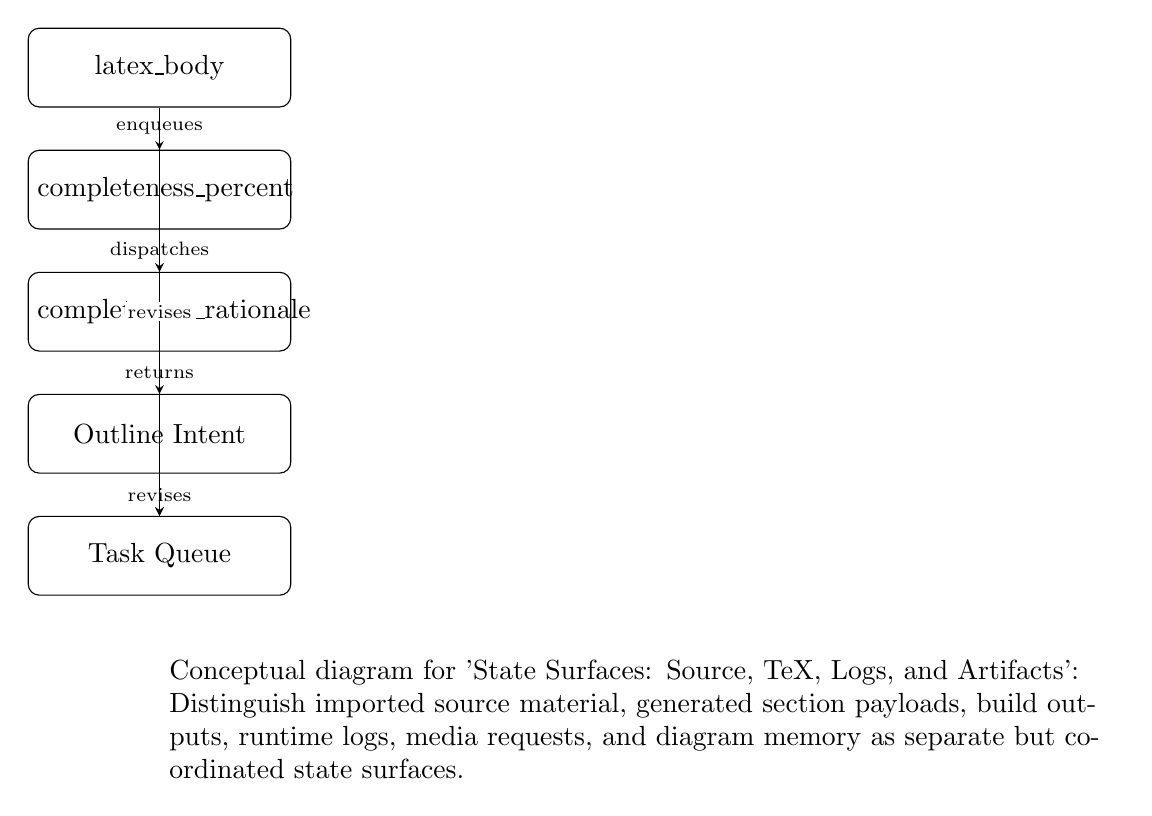
\begin{tikzpicture}[>=stealth, node distance=2.2cm,
  concept/.style={draw, rounded corners, align=center, text width=3.1cm, minimum height=1cm},
  relation/.style={font=\scriptsize, fill=white, inner sep=1pt}]
\node[concept] (n1) at (0,0.0) {latex\_body};
\node[concept] (n2) at (0,-1.55) {completeness\_percent};
\node[concept] (n3) at (0,-3.1) {completeness\_rationale};
\node[concept] (n4) at (0,-4.65) {Outline Intent};
\node[concept] (n5) at (0,-6.2) {Task Queue};
\draw[->] (n1) -- node[relation] {enqueues} (n2);
\draw[->] (n2) -- node[relation] {dispatches} (n3);
\draw[->] (n3) -- node[relation] {returns} (n4);
\draw[->] (n4) -- node[relation] {revises} (n5);
\draw[->] (n1) -- node[relation] {revises} (n5);
\node[align=left, text width=12cm, anchor=north west] at (0,-7.4) {Conceptual diagram for 'State Surfaces: Source, TeX, Logs, and Artifacts': Distinguish imported source material, generated section payloads, build outputs, runtime logs, media requests, and diagram memory as separate but coordinated state surfaces.};
\end{tikzpicture}

\caption{Conceptual diagram for ``State Surfaces: Source, TeX, Logs, and Artifacts'': Distinguish imported source material, generated section payloads, build outputs, runtime logs, media requests, and diagram memory as separate but coordinated state surfaces.}
\label{fig:state-surfaces}
\end{figure}


% CBM-SECTION-END:ch02_sec03_state_surfaces

\section{From Intake to Outline}

\subsection{Conversational Intake}

% CBM-SECTION-START:ch03_sec01_conversation:Conversational Intake

A conversational intake is the first structured exchange between the author and the book machine. Its purpose is to turn a loose writing idea into a machine-readable project brief that can drive outline generation, section planning, and later editorial work. Rather than asking for a finished manuscript, the system asks a small bank of targeted questions that establish the book's identity, scope, and production constraints.

The intake begins with the title. The title is not merely a label; it is the anchor for the work object, the repository layout, and the eventual compiled artifact. From there, the system asks for the purpose of the book: what the author wants the book to explain, demonstrate, or accomplish. Purpose gives the outline its direction and helps distinguish a technical paper, a tutorial, a design memo, or a reflective essay.

The next questions identify the intended audience and the reader takeaway. Audience describes who the book is for, including their likely background and expectations. Reader takeaway states what a reader should understand, be able to do, or be persuaded of after finishing the book. These two fields are complementary: audience constrains the level of explanation, while takeaway clarifies the outcome the manuscript should produce.

The intake also captures voice and genre. Voice describes the authorial stance the system should preserve, such as formal, explanatory, experimental, or conversational. Genre identifies the kind of document being produced, such as a technical paper, proposal, handbook, or narrative report. Together, voice and genre shape the tone of the generated outline and the style of the section drafts that follow.

A separate design specification question records how the manuscript should be presented. This may include structural preferences, formatting expectations, diagram density, citation style, or other production constraints that affect the shape of the final artifact. The design spec is important because the book machine does not treat prose as isolated text; it treats prose as one coordinated artifact among outlines, references, diagrams, logs, and compiled outputs.

Finally, the intake asks about artifact structure. This question establishes how the work should be organized into chapters, sections, appendices, or other units, and it gives the system an initial sense of the manuscript's granularity. In practice, artifact structure becomes the scaffold for the canonical work object, the section payloads, and the repository files that hold the evolving draft.

Taken together, the question bank converts author intent into a durable starting state. It does not attempt to solve the whole writing problem at once. Instead, it captures the minimum information needed to normalize the project into a structured outline, so that later agents can draft sections, register references, request diagrams, and maintain coherence across the manuscript.

Figure~\ref{fig:ch03_sec01_conversation_intake} summarizes the intake as a linked sequence of questions that moves from identity to purpose, from purpose to audience and takeaway, and from there to voice, genre, design constraints, and artifact structure. That progression matters because it mirrors the way the system stabilizes a project: first by naming it, then by clarifying what it is for, and finally by constraining how it should be written and assembled.

\begin{figure}[htbp]
\centering
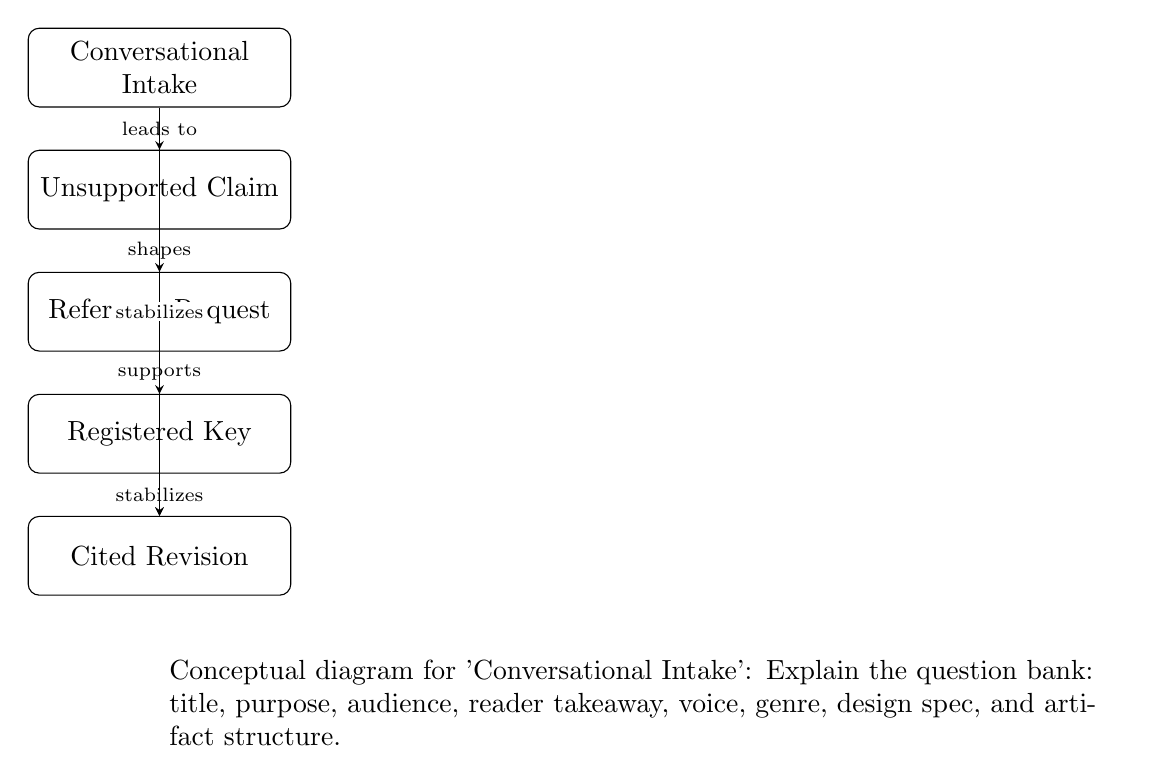
\begin{tikzpicture}[>=stealth, node distance=2.2cm,
  concept/.style={draw, rounded corners, align=center, text width=3.1cm, minimum height=1cm},
  relation/.style={font=\scriptsize, fill=white, inner sep=1pt}]
\node[concept] (n1) at (0,0.0) {Conversational Intake};
\node[concept] (n2) at (0,-1.55) {Unsupported Claim};
\node[concept] (n3) at (0,-3.1) {Reference Request};
\node[concept] (n4) at (0,-4.65) {Registered Key};
\node[concept] (n5) at (0,-6.2) {Cited Revision};
\draw[->] (n1) -- node[relation] {leads to} (n2);
\draw[->] (n2) -- node[relation] {shapes} (n3);
\draw[->] (n3) -- node[relation] {supports} (n4);
\draw[->] (n4) -- node[relation] {stabilizes} (n5);
\draw[->] (n1) -- node[relation] {stabilizes} (n5);
\node[align=left, text width=12cm, anchor=north west] at (0,-7.4) {Conceptual diagram for 'Conversational Intake': Explain the question bank: title, purpose, audience, reader takeaway, voice, genre, design spec, and artifact structure.};
\end{tikzpicture}

\caption{Conceptual diagram for Conversational Intake: the question bank captures title, purpose, audience, reader takeaway, voice, genre, design spec, and artifact structure.}
\label{fig:ch03_sec01_conversation_intake}
\end{figure}


% CBM-SECTION-END:ch03_sec01_conversation

\subsection{Outline Import and Normalization}

% CBM-SECTION-START:ch03_sec02_importer:Outline Import and Normalization

Legacy outlines enter the system through a normalization step that converts several human-friendly forms into the same canonical work representation. The goal is not merely to parse text, but to preserve authorial intent while making the structure machine-readable, comparable, and ready for downstream coordination. In practice, the importer accepts legacy YAML, markdown headers, numbered outlines, and even raw prose notes, then rewrites them into the work-oriented YAML used by the rest of the repository.

The normalization process begins by identifying the source shape. A legacy YAML file may already contain nested nodes, titles, and summaries, but its field names, nesting conventions, or metadata layout may differ from the current schema. Markdown sources usually encode structure implicitly through heading levels, list indentation, and emphasis. Numbered outlines often express hierarchy through numbering patterns such as 1, 1.1, and 1.1.1. Raw text may contain only paragraphs or loosely separated notes, requiring the importer to infer section boundaries from formatting cues and surrounding context. Each of these inputs is treated as a different surface form of the same underlying authorial plan.

Normalization then maps the imported material into canonical work YAML. At the top level, the importer establishes the work root and ensures that the document has the fields expected by the rest of the system: title, summary, intent, metadata, and a recursive structure of chapters, sections, and subsections. Imported headings become structural nodes with stable identifiers and explicit numbers. Free-form notes are attached as summaries or content files where appropriate, rather than left as ambiguous inline text. When the source already contains a usable hierarchy, the importer preserves that hierarchy while regularizing names, numbering, and field placement so that later agents can reason over it consistently.

A key part of the process is structural normalization. Markdown heading depth is translated into the book's recursive outline tree, with heading levels converted into chapter, section, or subsection nodes as needed. Numbered outlines are similarly converted by reading the numbering as a hierarchy signal rather than as presentation text. If the source uses mixed conventions, the importer resolves them into a single tree and records the result in a form that can be traversed uniformly. This makes it possible for later stages to compare sibling sections, detect missing dependencies, and generate section payloads without special-case parsing for each source format.

The importer also normalizes content boundaries. Some legacy sources place prose directly under headings, while others mix outline text with draft paragraphs or editorial notes. The canonical form separates structure from payload: the outline describes what exists, and the section content file or section body carries the prose that belongs to that node. This separation is important because the system treats the outline as durable project state, while section payloads are generated or revised independently. By moving imported text into the appropriate structural slot, the importer prevents accidental duplication and makes later revisions easier to target.

When the source is underspecified, normalization favors conservative preservation over invention. Raw text that cannot be confidently split into multiple sections should remain grouped rather than being over-partitioned. Ambiguous labels should be retained in a way that allows human review. The importer should not fabricate missing claims, dependencies, or metadata; instead, it should produce the most faithful canonical representation possible and leave unresolved gaps visible for later editorial work. In this sense, normalization is a migration step, not a creative rewrite.

The output of import is therefore a canonical work YAML file that can serve as the system's shared source of truth. Once normalized, the outline can be consumed by section agents, gardener checks, reference workflows, and build tooling without needing to know whether the project began as a legacy YAML tree, a markdown document, a numbered outline, or a block of raw notes. The importer turns heterogeneous author input into a stable project object, and that stability is what allows the rest of the machine to coordinate around a single representation.

In the repository's workflow, this section sits between conversational intake and repository layout. Conversational intake captures intent from the author; outline import converts preexisting material into the same canonical shape; repository layout then determines where the resulting work object, section payloads, logs, and artifacts live. Together, these steps define the path from informal source material to a structured book project that the rest of the Codynamic Book Machine can maintain.

\begin{figure}[htbp]
\centering
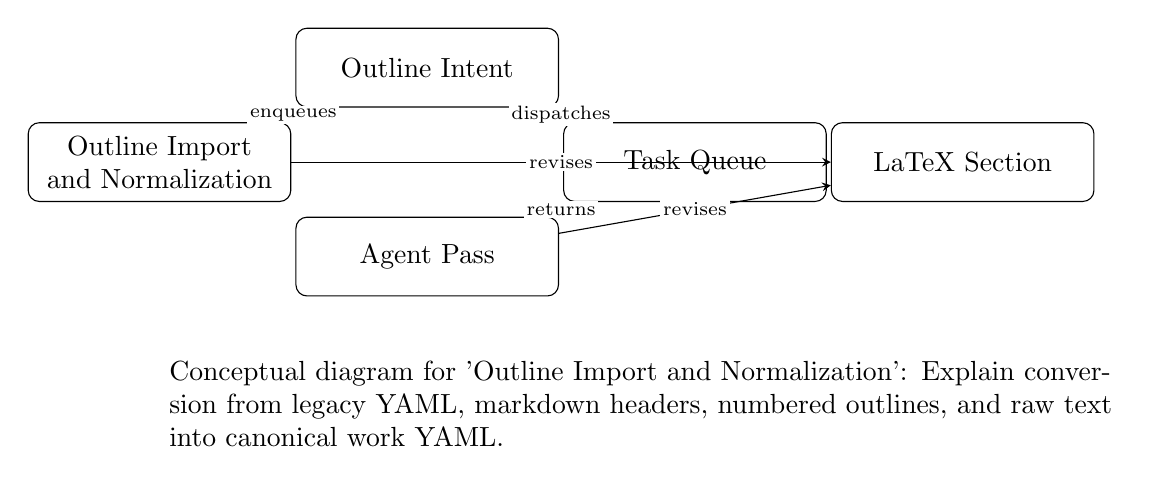
\begin{tikzpicture}[>=stealth, node distance=2.2cm,
  concept/.style={draw, rounded corners, align=center, text width=3.1cm, minimum height=1cm},
  relation/.style={font=\scriptsize, fill=white, inner sep=1pt}]
\node[concept] (n1) at (0,0) {Outline Import and Normalization};
\node[concept] (n2) at (3.4,1.2) {Outline Intent};
\node[concept] (n3) at (6.8,0) {Task Queue};
\node[concept] (n4) at (3.4,-1.2) {Agent Pass};
\node[concept] (n5) at (10.2,0) {LaTeX Section};
\draw[->] (n1) -- node[relation] {enqueues} (n2);
\draw[->] (n2) -- node[relation] {dispatches} (n3);
\draw[->] (n3) -- node[relation] {returns} (n4);
\draw[->] (n4) -- node[relation] {revises} (n5);
\draw[->] (n1) -- node[relation] {revises} (n5);
\node[align=left, text width=12cm, anchor=north west] at (0,-2.4) {Conceptual diagram for 'Outline Import and Normalization': Explain conversion from legacy YAML, markdown headers, numbered outlines, and raw text into canonical work YAML.};
\end{tikzpicture}

\caption{Conceptual diagram for ``Outline Import and Normalization'': Explain conversion from legacy YAML, markdown headers, numbered outlines, and raw text into canonical work YAML.}
\end{figure}


% CBM-SECTION-END:ch03_sec02_importer

\subsection{Book Repository Layout}

% CBM-SECTION-START:ch03_sec03_repository:Book Repository Layout

The Codynamic Book Machine keeps its working state in a repository that is intentionally split across a small number of durable surfaces. Rather than treating the manuscript as a single mutable file, the system separates outline structure, section source material, generated \TeX{} payloads, reference data, runtime logs, build outputs, media requests, diagram memory, and artifact registries. That separation is not incidental; it is what allows the book to be inspected, revised, rebuilt, and audited without collapsing authorial intent into a single opaque artifact.

At the top of the repository sits the outline and work definition. This is the canonical description of the book: its title, metadata, recursive structure, dependencies, and section inventory. The outline is the source of truth for what exists in the manuscript and how the manuscript is organized. Each chapter and section is represented as a structured node with an identifier, a number, a title, and a content file path. In practice, this means that the repository can answer two distinct questions at once: what the book is about, and where the editable payload for each part lives.

Section source files form the next layer. These files preserve imported notes, normalized source text, or other upstream material that informed a section before it was rendered into final prose. They are useful as a trace of provenance and as a staging area for conversion work. A section agent reads the source material, the outline intent, and the surrounding context, then writes the generated \TeX{} body to the section payload file for that section. The payload is the authored output, while the source file remains the record of what was imported or supplied.

The generated \TeX{} payloads are stored separately from the source material so that the manuscript can be assembled from many independently produced sections. This makes local revision possible without rewriting the whole book. A section payload should contain only the body content for that section, not the document preamble or wrapper commands. The assembly step later combines these payloads into the compiled manuscript. Keeping payloads isolated also makes it easier to compare drafts, attribute changes, and repair a single section without disturbing the rest of the document.

References are managed as a shared repository resource rather than as ad hoc citations embedded in arbitrary drafts. The bibliography file is the canonical store for registered citation keys, and section agents are expected to use only keys that have already been registered. When a section needs support that is not yet available, the section agent must request research or reference registration instead of inventing a citation. This keeps the manuscript honest about its evidentiary basis and makes citation support a coordinated task rather than a hidden authoring shortcut.

Logs provide the runtime memory of the system. They record task execution, agent messages, callbacks, and other durable traces of coordination. Because the system is message-driven, the logs are not merely diagnostic; they are part of the manuscript's operational history. A reader or maintainer can inspect them to understand why a section changed, which agent acted, what prompt or callback was involved, and how a revision was triggered. In that sense, the logs are a provenance layer for the authoring process itself.

Build artifacts capture the compiled state of the manuscript. These include generated \TeX{} outputs, PDFs, and any intermediate files produced during assembly or repair. They are distinct from the section payloads because they represent the result of combining many source surfaces into a single deliverable. When compilation fails, the build artifacts and logs together provide the evidence needed to repair the relevant section or adjust the assembly process. The compiled outputs are therefore not just publication products; they are also feedback signals for the authoring system.

Media requests and diagram memory extend the repository beyond text. When a section would benefit from a visual, the section agent can request a diagram rather than fabricating one inline. The request records the section context, the purpose of the figure, and the conceptual structure that the diagram should express. The diagram agent then creates the asset and returns a callback with a path and insertion hint. Diagram memory preserves the rationale for each generated figure, including its purpose, layout, nodes, edges, and distinctness from prior diagrams. This prevents the repository from accumulating redundant visuals and makes diagram generation a managed part of the manuscript's state.

Artifact registries tie these surfaces together. They provide a durable index of what has been created, where it lives, and how it should be used. A registry can point from a section identifier to its payload file, from a diagram request to its generated asset, or from a build to its output files and logs. In effect, the registry is the book's map: it lets agents and maintainers navigate the repository without guessing where a given artifact belongs.

Taken together, these repository layers make the book machine inspectable. Outline files define structure, source sections preserve upstream material, \TeX{} payloads hold generated prose, references support claims, logs preserve runtime history, build artifacts show compiled results, media requests and diagram memory manage visuals, and registries connect the whole system. The repository layout is therefore not just a file organization scheme; it is the operational boundary that keeps the manuscript coherent while many agents work on it at once.

Figure~\ref{fig:ch03_sec03_repository_layout} summarizes the repository as a set of coordinated surfaces rather than a single monolithic manuscript file. The outline anchors structure, section sources feed drafting, payloads store authored prose, and the registry layer links the resulting artifacts back to their origins.

\begin{figure}[htbp]
\centering
\input{media/diagrams/ch03_sec03_repository__media_req_cfc0a0a05ee9.tikz}
\caption{Conceptual diagram for Book Repository Layout: outline files, source sections, \TeX{} payloads, references, logs, build artifacts, media requests, diagram memory, and artifact registries.}
\label{fig:ch03_sec03_repository_layout}
\end{figure}


% CBM-SECTION-END:ch03_sec03_repository

\section{Agents, Tasks, and Runtime Memory}

\subsection{Agent Roles}

% CBM-SECTION-START:ch04_sec01_agent_roles:Agent Roles

The Codynamic Book Machine divides authoring work among a small set of specialized agents, each with a narrow responsibility and a clear handoff boundary. That division is not incidental: it is the mechanism that keeps outline intent, prose generation, editorial maintenance, references, diagrams, design, and compilation aligned as the manuscript evolves.

At the top of the runtime is the hypervisor, which supervises the whole project and coordinates work across agents. It receives high-level intent, starts section work, and escalates cross-cutting issues when a local fix is not enough. In practice, the hypervisor acts as the system's orchestration layer: it knows which section is being worked on, which tasks are pending, and when a callback or repair request should be routed to a specialist rather than handled inline.

The outlining and intake functions translate author intent into a structured work object. They are responsible for turning a topic, audience, and desired scope into a canonical outline that can be decomposed into chapters, sections, and subsections. Once the outline exists, it becomes the shared reference point for all downstream agents. Section agents do not invent the book's structure; they interpret and realize the structure that the outline already declares.

Section drafting is the responsibility of the section agents. Each section agent owns one section payload at a time and writes the \LaTeX{} body for that section only. Its job is to convert outline intent, imported source material, and runtime feedback into coherent prose that fits the surrounding chapter. Section agents also participate in the system's coordination protocol: they inspect their own section in context, choose among queued tasks, respond to callbacks, and revise their text when the gardener, references agent, diagram agent, or design agent identifies a needed change.

The gardener is the editorial maintenance agent. Rather than waiting for a human editor to notice drift, the gardener continuously checks the manuscript for repeated claims, thin transitions, missing definitions, unsupported assertions, and inconsistencies between a section and its neighbors. When it finds a local issue, it can request a targeted revision from the relevant section agent. When it finds a broader mismatch, it escalates the problem so the hypervisor can coordinate a wider repair. In this way, gardening functions as proactive editorial control rather than passive validation.

Reference support is handled by the references agent. It owns the shared bibliography and the canonical record of registered citation keys, which means section agents do not edit the bibliography directly. Instead, when a section needs support for a claim or a definition that is not already registered, the section agent must request research or hand off the missing support to the references agent. This separation keeps citation management centralized and prevents ad hoc bibliography drift. Section agents are expected to cite only registered keys, and to verify that a key exists before using it in the section text.

Diagram work is routed through the diagram agent. Section agents may propose diagrams when a visual would materially improve the explanation, but they do not fabricate diagram assets or paths. Instead, they send a structured request describing the section-specific concept that needs visualization, the purpose of the figure, and the relationships it should show. The diagram agent then creates the asset and returns a callback with the media path and inclusion hint. This keeps visual design distinct from prose drafting while still allowing the section to benefit from targeted illustrations.

Document design is a separate concern from section authorship. The design agent reviews the compiled manuscript as a document, not as isolated sections, and can flag layout, readability, or presentation issues that are better addressed at the document level than in a single section payload. That distinction matters because some problems are local to a paragraph, while others concern the overall shape of the paper, the balance of sections, or the consistency of the final artifact.

Finally, assembly turns the distributed work of the agents into a compiled paper. The assembler consumes the section payloads, bibliography, media assets, and build configuration, then produces the durable outputs that readers actually see. Assembly is the point at which the system's separate artifacts become a single document, but it is not the point at which authorship ends. If compilation exposes an error or a mismatch, the result is routed back into the agent workflow as a repair task, preserving the same durable, inspectable loop that governs drafting and revision.

Taken together, these roles form a layered division of labor: hypervision coordinates, outlining structures, section agents draft, gardening maintains coherence, references support claims, diagrams externalize relationships, design shapes presentation, and assembly produces the final artifact. The system's central design choice is that each responsibility has a specialist owner and a visible handoff, so the manuscript can evolve without losing track of who is responsible for what.


% CBM-SECTION-END:ch04_sec01_agent_roles

\subsection{Task Queues and Action Selection}

% CBM-SECTION-START:ch04_sec02_task_queues:Task Queues and Action Selection

Task queues are the mechanism that turns agent responsibility into executable work. Rather than asking a section agent to infer its next move from a free-form conversation, the system gives it a durable, ordered list of declared tasks. Each queued task records an \emph{action id}, a task context, a priority, a status, and the prompt or payload needed to perform the work. In practice, this means that a section agent can inspect its queue, identify which task corresponds to the current situation, and then execute that task without ambiguity.

The action id is the primary selector. It names the kind of work to be done, such as drafting a section, revising a section from feedback, responding to a callback, requesting research, or coordinating with a sibling agent. The task context narrows that action to the relevant section, claim, or artifact. For example, a task may point to a specific section id, a feedback message, a missing citation, or a diagram opportunity. The queue therefore separates \emph{what} kind of work is needed from \emph{where} that work applies.

Priority determines ordering when more than one task is available. Higher-priority tasks are chosen first, but only among tasks that are actually eligible to run. A section agent does not simply pick the oldest item in the queue; it evaluates the declared tasks against the current state of the section, the document, and any callback messages that have arrived. This keeps urgent repairs, explicit callbacks, and prerequisite work from being buried behind routine drafting tasks.

The prompt attached to a task is generated from the task context and the current document state. For a drafting task, the prompt may include the section title, summary, sibling section context, and the relevant outline path. For a revision task, it may include the feedback that triggered the revision and the exact constraints that must be preserved. For a research task, it may include the unsupported claim or missing definition that needs external support. The prompt is not a generic instruction; it is a task-specific working brief assembled from durable context.

Task status transitions make the queue observable. A task typically moves from queued to active when the agent begins work, and then to completed, failed, or blocked depending on the outcome. If a prerequisite is missing, the agent should not fabricate the missing material; instead, it should leave the task unresolved and queue or request the prerequisite work. This is especially important for citations, definitions, and file paths, where guessing would create hidden errors in the manuscript.

Section agents choose which declared task to run by matching the queue against the current situation. If the agent has been started manually, it first inspects the full document, its own section, the outline, registered references, and diagram opportunities, then uses that inspection to decide which task is the correct next action. If a callback message arrives, the callback is treated as work rather than as a passive notification. If the section needs a revision, the agent revises; if it needs research, the agent requests research; if it needs coordination, the agent responds to the sibling agent or hypervisor. The queue is therefore not just a list of jobs, but the runtime representation of editorial intent.

This selection process is constrained by declared task modes. A section agent should not invent a new action when an existing task already describes the needed work. It should also not ignore a callback in favor of a lower-value drafting task. The intended behavior is disciplined and local: inspect the queue, identify the task whose action id and context match the current state, and execute that task with the least possible drift.

In the Codynamic Book Machine, this discipline matters because the manuscript is not edited by hidden side effects. Every meaningful change is routed through a task, every task has a status, and every status change can be inspected later. The result is a section workflow that is both autonomous and auditable: the agent can act on its own, but it does so by selecting from explicit work items rather than by improvising outside the queue.

A concrete way to read this section is as a decision rule for the section agent. If the queue contains a direct drafting task for the current section, that task is the default choice. If a callback has arrived, the callback takes precedence because it represents a concrete unresolved event. If the section is missing a prerequisite, such as a citation key or a diagram path, the agent should not continue as if the prerequisite existed; it should route the missing work to the appropriate specialist workflow and mark the current task as blocked or pending. That ordering keeps the runtime honest about what can actually be completed now.

The same rule also explains why the queue is durable rather than conversational. A chat exchange can suggest what should happen next, but the queue records what the system has formally committed to do. That distinction lets the hypervisor, the section agent, and later maintenance passes inspect the same work list and agree on which action is active, which one is waiting, and which one has already been resolved. In other words, the queue is the manuscript's executable to-do list, not just a memory aid.

For this chapter, the task-queue model also provides the bridge to the next section on messages and callbacks. Tasks say what should happen; messages say what was said; callbacks convert message events into new work. Together, they form the runtime loop that keeps the manuscript moving without losing track of responsibility.

\begin{figure}[htbp]
\centering
\input{media/diagrams/ch04_sec02_task_queues__media_req_df83c09eb86c.tikz}
\caption{Conceptual diagram for task queues and action selection.}
\end{figure}


% CBM-SECTION-END:ch04_sec02_task_queues

\subsection{Messages, Callbacks, and the Inter-Agent Chat Log}

% CBM-SECTION-START:ch04_sec03_messages:Messages, Callbacks, and the Inter-Agent Chat Log

Messages are the runtime substrate that makes the rest of the agent system legible. Tasks describe what an agent should do, but messages describe what actually happened: a request was routed, a callback arrived, a self-check was queued, or the hypervisor observed a line of chat that had not yet been processed. In this system, the message stream is not an incidental log; it is part of the manuscript's operational memory.

The basic unit is a routed message between named agents. A message records a sender, a recipient, and a human-readable payload, and it is rendered in an append-only chat log in the form \texttt{from\_agent --\textgreater{} to\_agent: message}. That format is intentionally simple. It can be scanned by a human, parsed by tooling, and replayed as evidence of how a section was produced. Because the log is append-only, later work does not erase earlier coordination; it accumulates beside it.

Routed messages serve several distinct purposes. Some are direct work requests, such as asking a section agent to draft or revise prose. Others are coordination messages between sibling agents, for example when one section agent needs a neighboring section to align terminology or avoid duplication. Still others are callback messages that report the result of a completed action. The system treats these callbacks as first-class work items rather than as passive notifications.

A particularly important callback type is \texttt{process\_message}. When an agent receives a routed message that requires interpretation, the runtime can enqueue a \texttt{process\_message} task so the recipient handles the message explicitly. This makes message handling durable and inspectable. Instead of assuming that a message was read immediately and correctly, the system records the act of processing as a task with its own status, prompt, and outcome. In practice, this means that a callback can become the next concrete unit of work: revise a section from feedback, request research, coordinate with a sibling, or simply acknowledge receipt.

Self-messages are another useful pattern. An agent may send a message to itself when it needs to preserve a decision, stage a follow-up action, or convert a reflective note into queued work. For section agents, self-messages often support planning: after inspecting the outline, the section payload, registered references, and diagram opportunities, the agent can queue a self-addressed plan that becomes visible in the same durable chat stream as external coordination. This keeps internal deliberation from disappearing into hidden state.

The chat log is therefore both operational and readable. It shows the sequence of interactions that led to a draft, but it also exposes the system's intermediate reasoning in a form that can be audited later. The hypervisor can inspect unprocessed chat lines directly, which gives it access to the live edge of coordination rather than only to completed task records. That access matters when the hypervisor needs to intervene, reconcile competing actions, or detect that a callback has arrived but has not yet been handled by the intended agent.

This separation between messages and tasks is deliberate. Tasks describe durable obligations with status transitions; messages describe the conversational surface through which those obligations are negotiated, delegated, and confirmed. The result is a runtime in which coordination is visible at two levels at once: the queue shows what must be done, and the chat log shows how the system talked itself into doing it.

The same distinction also clarifies why the system keeps message handling explicit. A routed message may be informative, directive, or corrective, but it does not by itself change the state of the manuscript. Only when the recipient processes it does the message become operationally meaningful. That extra step is what makes the chat log useful as a source of provenance: one can see not only that a request was issued, but also that it was acknowledged, interpreted, and converted into a concrete follow-up action.

In practice, this means the inter-agent chat log is not merely a transcript of conversation. It is a coordination ledger. It records the handoff from one agent to another, the return path of callbacks, the internal notes that agents preserve for themselves, and the unprocessed lines that remain visible to the hypervisor. Taken together, those traces make the runtime inspectable without making it opaque to the agents that depend on it.

The section is intentionally self-contained and does not require a visual to carry its argument, so no diagram is requested here.


% CBM-SECTION-END:ch04_sec03_messages

\subsection{Introspective Starts}

% CBM-SECTION-START:ch04_sec04_introspective_start:Introspective Starts

Starting a section agent should begin with an explicit inspection pass rather than immediate prose generation. In practice, that means the agent first reads the full document outline to recover the chapter-level argument, then checks the selected section against its sibling sections so the local transition fits the surrounding narrative. It also inspects the section payload itself, the registered reference set, and any diagram opportunities before it writes a draft. This front-loaded review keeps the section aligned with the book's schema-first workflow and prevents the agent from drafting in isolation.

The inspection pass is not merely passive reading. It is a deliberate inventory of the work state that the agent will need in order to act responsibly: the current outline node, the section summary, any imported source material, the available citation keys, and the visual affordances of the section. For a section agent, those inputs define the boundaries of what can be stated directly, what must be deferred to a reference handoff, and whether a diagram would materially improve comprehension. The result is a small but important planning step that turns a generic start-up event into a concrete work plan.

That planning step is especially important because the section agent is not starting from a blank page in the abstract; it is starting from a specific place in a larger manuscript. The chapter has already established the agent roles, the task queue model, and the message-and-callback runtime. An introspective start extends that machinery into the first moment of section work by making the agent ask, in effect, ``What is the document trying to do, what is this section supposed to contribute, and what support is already available?'' Only after those questions are answered does drafting become a responsible next step.

After that inspection, the agent queues a self-addressed plan message. This message enters the same durable task system used for ordinary work, so the plan is visible, inspectable, and replayable like any other task. The self-message can summarize the intended drafting strategy, note missing references, record whether a diagram request is warranted, and identify the next action to execute. In other words, the agent does not silently ``think ahead''; it externalizes the plan into the queue so the runtime can track how the section moved from initialization to drafting.

That pattern matters because it makes section startup part of the manuscript's observable state. A section does not begin as an opaque burst of generation; it begins as a documented decision to inspect, assess, and then act. The introspective start therefore serves two purposes at once: it gives the section agent enough context to draft well, and it leaves behind a durable trace that explains why the draft took the shape it did. In a codynamic system, even the first step of writing is itself a managed artifact.

The section also fits naturally beside the surrounding runtime discussion. The preceding sections explain how tasks are queued and how messages move through the system; this section narrows that machinery to the moment a section agent wakes up and decides what to do first. The emphasis is not on a special new capability, but on disciplined sequencing: inspect the document, inspect the section, inspect the available support, then queue the plan that will govern the next action.

Seen that way, the introspective start is a small control loop rather than a ceremonial preface. It reduces the chance that a section agent will draft against stale assumptions, overlook a sibling section's contribution, or miss a missing citation that should have been routed elsewhere. It also makes the agent's first move legible to the rest of the system: the hypervisor can see that the section has entered a planning phase, the gardener can later interpret the resulting draft in light of the inspection, and the references and diagram workflows can be invoked only when the section actually needs them.

The section is intentionally self-contained and does not require a visual to carry its argument, so no diagram is requested here.


% CBM-SECTION-END:ch04_sec04_introspective_start

\section{Gardening as Editorial Control}

\subsection{The Maintenance Cycle}

% CBM-SECTION-START:ch05_sec01_maintenance_cycle:The Maintenance Cycle

The gardener's maintenance cycle is the recurring editorial routine that keeps the manuscript aligned as the surrounding work changes. Rather than waiting for a build failure or a human complaint, the gardener periodically inspects the current state of the repository and compares each affected section against the rest of the book. The goal is not merely to detect errors, but to identify the smallest useful editorial action that will restore coherence.

A maintenance pass begins with change inspection. The gardener reviews newly edited sections, updated outlines, revised prompts, and any downstream artifacts that may have been invalidated by those changes. This first pass is intentionally broad: a local edit can alter terminology, dependencies, or claims in sections that do not themselves contain the edit. The gardener therefore treats the manuscript as a connected system rather than a set of isolated files.

After identifying the changed region, the gardener compares the section against several reference points. The parent section provides the higher-level argument and establishes what the subsection is supposed to contribute. Sibling sections provide immediate narrative context and help reveal duplication, gaps, or inconsistent terminology. Declared dependencies indicate which earlier material the section relies on, while downstream uses show where the section's concepts, definitions, or phrasing are reused later in the book. These comparisons let the gardener distinguish a purely local wording issue from a structural mismatch that will propagate elsewhere.

This comparison step is what makes the maintenance cycle editorial rather than mechanical. A section may be internally well formed yet still repeat a claim already made in a sibling, omit a transition that the parent section needs, or introduce a term that later sections assume without definition. The gardener looks for those mismatches and classifies them by scope. Some issues can be repaired by a single section agent. Others require coordinated revisions across multiple sections. Still others are not prose problems at all, but missing support that must be routed to the references agent.

Once the gardener has identified the relevant issue class, it queues targeted work instead of rewriting the manuscript wholesale. A repeated claim may become a revision request to the section that introduced it. A thin transition may be assigned to the section that needs a bridging sentence. A missing definition may be routed to the section where the term first appears, or to the references agent if the term requires external support. This targeted routing keeps the maintenance cycle small, inspectable, and reversible.

The recurring nature of the cycle matters as much as the checks themselves. Because the manuscript evolves through many small agent actions, coherence cannot be enforced only at the end of drafting. The gardener therefore acts as a standing editorial process: inspect, compare, classify, and queue. In effect, it keeps the book in a state of continuous maintenance, where local edits are evaluated against the broader structure before they harden into global drift.

This section's role in the larger chapter is to establish that gardening is not a passive validation step. It is an active control loop that watches the manuscript's moving parts, compares them across structural boundaries, and dispatches the smallest corrective task that will preserve the book's internal consistency. The next section separates those local revision requests into concrete categories, showing how repeated claims, thin transitions, missing definitions, and unsupported assertions each route to a different repair path.


% CBM-SECTION-END:ch05_sec01_maintenance_cycle

\subsection{Editorial Checks and Revision Requests}

% CBM-SECTION-START:ch05_sec02_editorial_checks:Editorial Checks and Revision Requests

This section distinguishes the kinds of editorial problems the gardener can resolve locally from the kinds that require specialist handoff. Not every defect in a draft is the same defect: some passages repeat an idea that has already been established, some move too abruptly between claims, some introduce a term that has not yet been defined, and some assert a fact that the manuscript does not yet support. The maintenance cycle in Section~5.1 treats these as different signals because they route to different agents and different repair strategies.

Repeated claims are usually the easiest to detect. When two adjacent sections restate the same point in nearly the same language, the problem is not factual correctness but redundancy. The gardener can mark the overlap and ask the relevant section agent to compress or remove the repeated material. In practice, this is a local revision request: the section agent revises its own payload so the manuscript keeps one clear statement instead of several near-duplicates. The goal is not to eliminate all reinforcement, but to avoid prose that feels circular or padded.

Thin transitions are a related but distinct issue. A section may be individually correct and still read as if one paragraph has been pasted next to another without connective tissue. In that case, the gardener does not ask for new evidence; it asks for a better bridge. The section agent may need to add a sentence that explains why the next concept follows from the previous one, or to restate the local purpose of the section so the reader can track the argument. These requests are editorial rather than substantive: they improve continuity, pacing, and reader orientation without changing the underlying claim.

Missing definitions require a different response. If a section uses a term that the outline or surrounding prose has not yet defined, the gardener should not let the term drift into vague usage. Instead, it routes the issue back to the section agent responsible for the local context, or to the section that owns the concept if the definition belongs elsewhere in the outline. The repair may be as simple as adding a short definition where the term first appears, or as involved as coordinating with a sibling section so the definition is introduced before the term is reused. The important point is that undefined terminology is a structural gap, not merely a stylistic flaw.

Unsupported assertions are the category that most clearly requires reference support. When a section makes a claim that depends on external evidence, implementation details, or a specific documented behavior, the gardener checks whether the manuscript already has a registered citation key that can support it. If the claim is already backed by a registered source, the section agent can cite it directly. If not, the issue is escalated to \texttt{references\_agent} through a structured request for research or citation registration. The section agent should not invent a citation key or leave a fabricated reference in place. It should either wait for the registered key or revise the prose so that it no longer overstates what the manuscript can currently support.

These categories route differently because they imply different kinds of repair. Repetition and thin transitions are usually handled by the owning section agent, since they are matters of local prose shape. Missing definitions may also be handled locally, but they often require coordination with a sibling section or an earlier chapter if the definition belongs in a shared conceptual foundation. Unsupported assertions, by contrast, are routed toward \texttt{references\_agent} whenever the manuscript needs a source that is not yet registered. That handoff preserves the separation between prose revision and bibliography ownership.

The gardener's job is therefore not simply to flag problems, but to classify them. A repeated claim asks for compression. A thin transition asks for connective prose. A missing definition asks for conceptual repair. An unsupported assertion asks for citation support or for the claim to be softened until support exists. By separating these cases, the editorial loop keeps revision requests precise, keeps section agents focused on the work they own, and keeps \texttt{references\_agent} responsible for the evidence trail that underwrites the manuscript.

In the broader maintenance cycle, this classification also prevents unnecessary escalation. A section that merely repeats itself does not need a bibliography search. A section that lacks a definition does not need a global rewrite. And a claim that lacks support should not be disguised as a stylistic issue. The manuscript stays coherent when each defect is routed to the agent best suited to repair it, and this section names the routing logic that makes that possible.

A useful way to read the gardener's classification is as a small decision tree. If the text says the same thing twice, the fix is compression. If the text jumps too quickly, the fix is a transition. If the text uses a term before the reader can place it, the fix is a definition or a coordination request. If the text reaches beyond what the manuscript can currently justify, the fix is either a citation or a more cautious claim. That distinction matters because it keeps editorial work proportional: the gardener does not turn every problem into a research task, and it does not turn every research need into a prose-only edit.

This routing logic also makes revision requests easier to interpret downstream. A section agent receiving a note about repetition knows to shorten or merge material. A note about a thin transition tells the agent to add connective prose rather than new content. A note about a missing definition signals that the section may need to borrow conceptual groundwork from a sibling or earlier section. And a note about an unsupported assertion tells the agent to either cite a registered source or narrow the claim until support is available. The request itself therefore carries the repair strategy, which reduces ambiguity and keeps the editorial loop efficient.

Taken together, these checks show that gardening is not a generic quality filter. It is a classification layer that separates prose shape, conceptual completeness, and evidentiary support. That separation is what lets the system route work to the right owner: section agents handle local revision, sibling coordination resolves shared terminology, and \texttt{references\_agent} owns the evidence trail. The result is a manuscript that can be corrected without collapsing every issue into the same kind of task.

One practical implication is that the gardener can keep a revision note narrowly scoped. If the problem is repetition, the note can point to the duplicated sentence and ask for compression. If the problem is a thin transition, the note can ask for one bridging sentence rather than a wholesale rewrite. If the problem is a missing definition, the note can identify the first occurrence of the term and ask whether the definition belongs here or in a sibling section. If the problem is an unsupported assertion, the note can either request a registered citation or ask the authoring agent to soften the claim until support is available. That specificity keeps the maintenance cycle efficient and reduces the chance that a local issue becomes a broad editorial detour.

In the context of this chapter, the section also sets up the next distinction: local editorial checks versus manuscript-level drift. The checks described here are the ones the gardener can usually resolve by targeting a single section or a small set of related sections. When the same issue spans multiple sections, the problem is no longer just a revision request; it becomes a coordination problem for the hypervisor. Section~5.3 takes up that broader escalation path.

\begin{figure}[htbp]
\centering
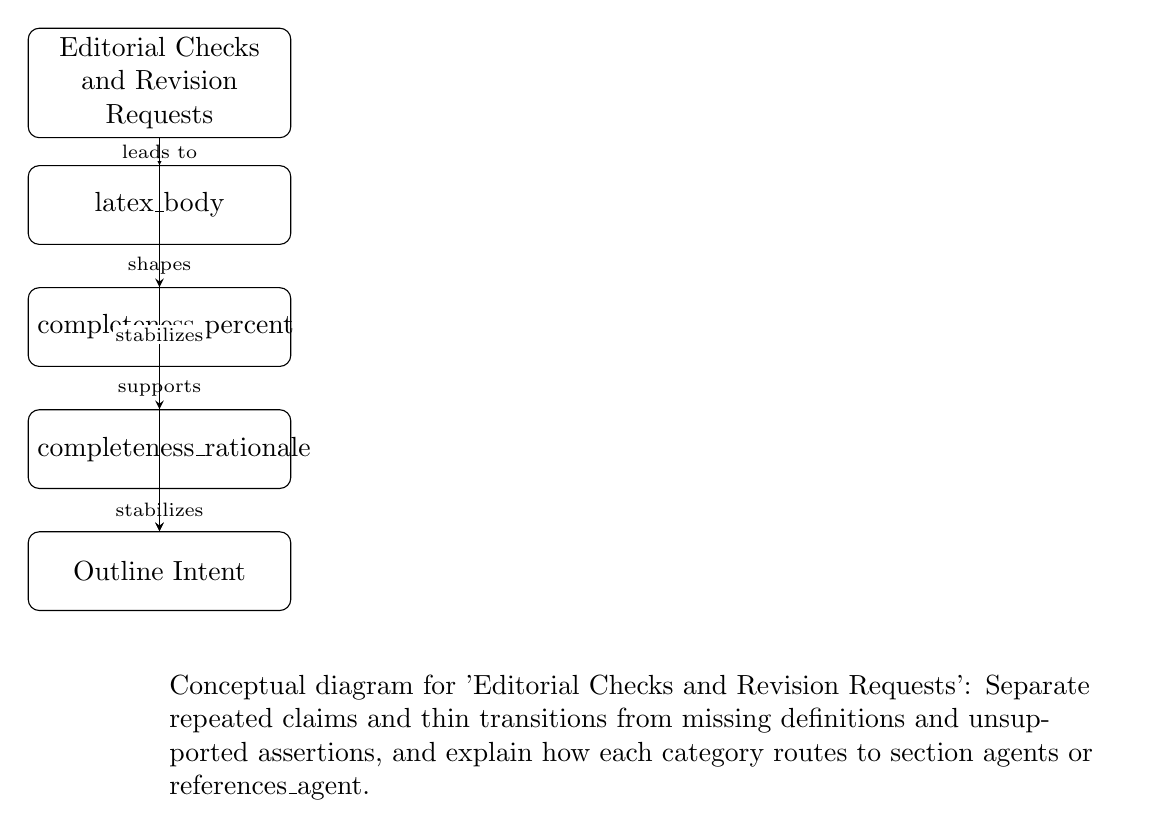
\begin{tikzpicture}[>=stealth, node distance=2.2cm,
  concept/.style={draw, rounded corners, align=center, text width=3.1cm, minimum height=1cm},
  relation/.style={font=\scriptsize, fill=white, inner sep=1pt}]
\node[concept] (n1) at (0,0.0) {Editorial Checks and Revision Requests};
\node[concept] (n2) at (0,-1.55) {latex\_body};
\node[concept] (n3) at (0,-3.1) {completeness\_percent};
\node[concept] (n4) at (0,-4.65) {completeness\_rationale};
\node[concept] (n5) at (0,-6.2) {Outline Intent};
\draw[->] (n1) -- node[relation] {leads to} (n2);
\draw[->] (n2) -- node[relation] {shapes} (n3);
\draw[->] (n3) -- node[relation] {supports} (n4);
\draw[->] (n4) -- node[relation] {stabilizes} (n5);
\draw[->] (n1) -- node[relation] {stabilizes} (n5);
\node[align=left, text width=12cm, anchor=north west] at (0,-7.4) {Conceptual diagram for 'Editorial Checks and Revision Requests': Separate repeated claims and thin transitions from missing definitions and unsupported assertions, and explain how each category routes to section agents or references\_agent.};
\end{tikzpicture}

\caption{Conceptual diagram for ``Editorial Checks and Revision Requests'': separate repeated claims and thin transitions from missing definitions and unsupported assertions, and show how each category routes to section agents or \texttt{references\_agent}.}
\end{figure}


% CBM-SECTION-END:ch05_sec02_editorial_checks

\subsection{Global Drift and Hypervisor Escalation}

% CBM-SECTION-START:ch05_sec03_global_drift:Global Drift and Hypervisor Escalation

The gardener does not treat every inconsistency as a local defect. When a change reveals a mismatch that spans multiple sections---for example, a definition that has shifted, a repeated claim that now appears in several places, or a transition that no longer matches the surrounding argument---the issue is escalated as \emph{global drift}. In that case, the gardener assembles a concise list of the affected section agents and forwards it to the hypervisor, rather than sending isolated revision requests one by one.

This escalation step matters because coordinated revision is a different problem from ordinary maintenance. A single section agent can repair a thin transition, add a missing explanation, or tighten a paragraph in place. But when the same conceptual change must be reflected across several sections, the manuscript needs a higher-level decision about ordering, scope, and consistency. The hypervisor is the agent that can see the affected set as a whole and direct the revision sequence so that one section does not silently reintroduce drift into another.

The gardener's report to the hypervisor is therefore structured around impact, not just symptoms. It identifies which section agents are implicated, what kind of mismatch has been detected, and why the issue cannot be resolved safely as a purely local edit. That list becomes the basis for coordinated follow-up: the hypervisor can route revision tasks to the relevant section agents, preserve the intended narrative order, and ensure that shared terminology, dependencies, and downstream references are updated together.

A useful way to think about this handoff is as a compact affected-agent set. The gardener is not merely saying that something is wrong; it is naming the manuscript region that must move together. For example, if a definition introduced in one section has been revised, the gardener may include the defining section, the sections that reuse the term, and the current section in the same escalation. The hypervisor can then decide whether the defining section should be revised first, whether dependent sections should wait for that revision, or whether the whole cluster should be updated in a single coordinated pass.

In practice, this makes global drift a manuscript-level control signal. Local editorial checks keep individual sections clean, but hypervisor escalation keeps the book coherent when the same change must propagate across the outline. The result is a maintenance loop that can distinguish between a paragraph-level repair and a coordinated revision campaign, using the gardener to detect the former and the hypervisor to orchestrate the latter. That distinction is what prevents a local fix from becoming a new source of inconsistency elsewhere in the chapter.

The section therefore closes the chapter's maintenance story by showing where ordinary gardening stops. Section-level revision is enough when the problem is isolated. Once the mismatch crosses section boundaries, the gardener stops patching piecemeal and hands the hypervisor a bounded list of affected agents so the revision can be scheduled as one coherent operation.

This section does not require a diagram: the core idea is the escalation rule itself, and the surrounding chapter already establishes the agent roles and maintenance cycle that make the handoff legible.


% CBM-SECTION-END:ch05_sec03_global_drift

\section{Specialist Handoffs: References and Diagrams}

\subsection{Reference Ownership and Citation Support}

% CBM-SECTION-START:ch06_sec01_references:Reference Ownership and Citation Support

The reference workflow is intentionally centralized so that citation state has a single owner. The shared bibliography file, \texttt{references/references.bib}, is maintained by \texttt{references\_agent} rather than by individual section agents. That division of responsibility prevents concurrent edits from fragmenting the bibliography, keeps citation keys canonical, and gives the system one place to register, validate, and update reference records.

Section agents therefore treat the bibliography as read-only support data. When drafting or revising a section, a section agent first checks the registered reference context and verifies that every citation key it intends to use already exists in \texttt{references/references.bib}. If a key is registered, the section can cite it directly with the house citation command or \texttt{\textbackslash cite\{key\}} as appropriate. If a key is not registered, the section agent does not invent a citation, guess at a source, or silently omit the support. Instead, it routes the gap into the reference workflow by requesting research or by sending a structured handoff to \texttt{references\_agent}.

That handoff is the mechanism that keeps unsupported claims visible. A missing citation, missing definition, or otherwise ungrounded statement becomes an explicit task rather than an implicit assumption. The section agent can queue a \texttt{do\_research\_on\_the\_web} task when the needed source is not yet known, then forward candidate bibliographic records to \texttt{references\_agent} for registration. Once \texttt{references\_agent} confirms the new keys, the section agent verifies that those keys are present in \texttt{references/references.bib} and only then revises the prose to use them.

This ownership model has two practical benefits. First, it keeps citation support auditable: every key used in a section can be traced back to a registered bibliography entry. Second, it keeps section drafting focused on prose rather than bibliography maintenance. The section agent is responsible for recognizing where support is needed and for integrating approved keys into the text, while \texttt{references\_agent} is responsible for the canonical reference store itself. In the Codynamic Book Machine, that separation is what turns citation management into a durable workflow instead of an ad hoc editing habit.

The same pattern also clarifies how reference support fits into the broader chapter. Section agents do not merely ask whether a claim sounds plausible; they check whether the manuscript already has the support needed to state it responsibly. If the support exists, they cite it. If it does not, they route the gap to the specialist workflow that can resolve it. That discipline keeps the manuscript honest about what is grounded in registered evidence and what still requires follow-up.

In the surrounding chapter, this section establishes the reference side of specialist handoffs. The next section extends the same pattern to diagrams: section agents may identify a visual need, but they must route the request through the diagram workflow and wait for a callback before inserting any asset path into the section payload.


% CBM-SECTION-END:ch06_sec01_references

\subsection{Diagram Requests and Callbacks}

% CBM-SECTION-START:ch06_sec02_diagram_requests:Diagram Requests and Callbacks

Section agents treat diagram work as a bounded post-revision activity rather than an open-ended design exercise. After a draft has been produced or revised, the agent may propose zero, one, or two diagrams if a visual would materially improve the section's explanation. This limit keeps diagramming focused on the smallest set of figures that clarify the local argument, rather than turning every section into a gallery of illustrations.

The diagram proposal step is also selective about where it applies. Front matter such as the title page, abstract, dedication, foreword, preface, table of contents, and acknowledgements is excluded from diagram requests. Those parts are meant to orient the reader, not to introduce technical workflows that benefit from a figure. Main content and back matter may request diagrams when a visual would help explain a process, relationship, or lifecycle.

When a diagram is warranted, the section agent does not invent a file path or assume that an asset already exists. Instead, it queues a \texttt{create\_diagram\_asset} task, or asks the hypervisor to queue that task on its behalf, with a concrete description of the needed figure. A useful request identifies the section, the requesting agent, the media type, and the purpose of the diagram. When possible, it also includes a diagram specification with three to five node labels, two to five labeled edges, and a suggested layout so the diagram agent can generate an asset that matches the section's argument.

The request is only the first half of the workflow. The section agent must then wait for the diagram agent's callback before inserting any media path into the \LaTeX{} payload. That callback arrives as a \texttt{process\_message} task and includes the generated media path together with a \LaTeX{} inclusion hint. Only after processing that callback should the section agent revise the section to include the figure reference or \texttt{\textbackslash includegraphics} command. This waiting step prevents the manuscript from pointing at missing assets and keeps the section payload synchronized with the durable diagram registry.

A concrete request makes the workflow easier to see. A section on task routing might ask for a compact flow diagram showing the revision pass, the diagram request decision, the queued asset task, and the callback that returns the path. The request would still stop at the handoff stage until the callback arrives, even if the diagram is obviously useful. That discipline keeps the prose, the task queue, and the media registry aligned.

In practice, diagram handling follows a disciplined sequence: revise the prose, decide whether a figure would add real explanatory value, queue at most two diagram requests, and then pause until the callback confirms the asset location. The result is a section that can describe its own visual needs without coupling itself to speculative file paths or premature inclusions. This section also sets up the neighboring discussion of diagram memory, where the returned asset is recorded with its purpose, nodes, edges, layout, and distinctness rationale so later work can tell whether a new request is genuinely new or merely redundant.


% CBM-SECTION-END:ch06_sec02_diagram_requests

\subsection{Diagram Agent Memory}

% CBM-SECTION-START:ch06_sec03_diagram_memory:Diagram Agent Memory

The diagram agent is not merely a renderer; it is a memory-bearing specialist that must make each new figure legible in the context of the figures that came before it. That requirement matters because diagram requests in this system are not isolated image-generation prompts. They are part of a continuing editorial conversation in which the section agent proposes a visual, the diagram agent produces an asset, and later section or gardener work may need to refer back to the same visual logic. If the diagram agent were prompted only with the current request, it could easily repeat an earlier layout, reuse the same conceptual structure under a different label, or generate a figure that is technically correct but redundant with an existing asset. Supplying prior diagram context reduces that drift by giving the agent a local memory of what has already been drawn and why.

That memory is also a coordination mechanism. The section agent does not ask for a diagram in the abstract; it asks for a diagram that serves a specific rhetorical purpose in a specific section. To preserve that purpose across callbacks, the diagram agent records the purpose, the node set, the labeled edges, the layout choice, the generated path, and the rationale for distinctness. Those fields capture both the content of the figure and the reason it exists. Purpose explains what the diagram is meant to clarify. Nodes and edges describe the conceptual structure the figure encodes. Layout records the spatial strategy used to make that structure readable. Path identifies the durable artifact that later section agents may include. Distinctness rationale explains how the new figure differs from earlier ones, which is essential when multiple diagrams live in the same chapter or when a later revision must decide whether a new request is genuinely new work or a duplicate of an existing asset.

This memory model supports two forms of editorial control. First, it helps the diagram agent avoid repetition. A chapter may need several diagrams, but they should not all restate the same relationship with only cosmetic changes. By comparing a proposed figure against prior diagram context, the agent can prefer complementary visuals: one diagram may show the runtime task flow, another may show the callback lifecycle, and a third may show how memory entries are registered and reused. Second, it helps the section agent reason about insertion. When a callback arrives with a media path and inclusion hint, the section agent can verify that the asset matches the intended purpose and that it is distinct from earlier figures before inserting it into the section payload.

The result is a small but important form of durable visual memory. The system does not treat diagrams as disposable images; it treats them as named artifacts with provenance, function, and relationships to sibling figures. That is why the diagram agent receives prior diagram context in its prompt and why it records each diagram's purpose, nodes, edges, layout, path, and distinctness rationale. Those records make the visual layer inspectable, prevent unnecessary duplication, and keep diagram generation aligned with the evolving manuscript rather than with a single isolated request.

The neighboring section on diagram requests explains the front end of this workflow: a section agent proposes a bounded visual need, waits for the callback, and only then inserts the returned path. This section explains the back end of the same workflow: once the asset exists, the diagram agent's memory keeps the figure intelligible across later revisions, sibling sections, and chapter-level maintenance. Together, the two sections define a complete visual handoff protocol in which request, generation, callback, and memory remain synchronized.

\begin{figure}[htbp]
\centering
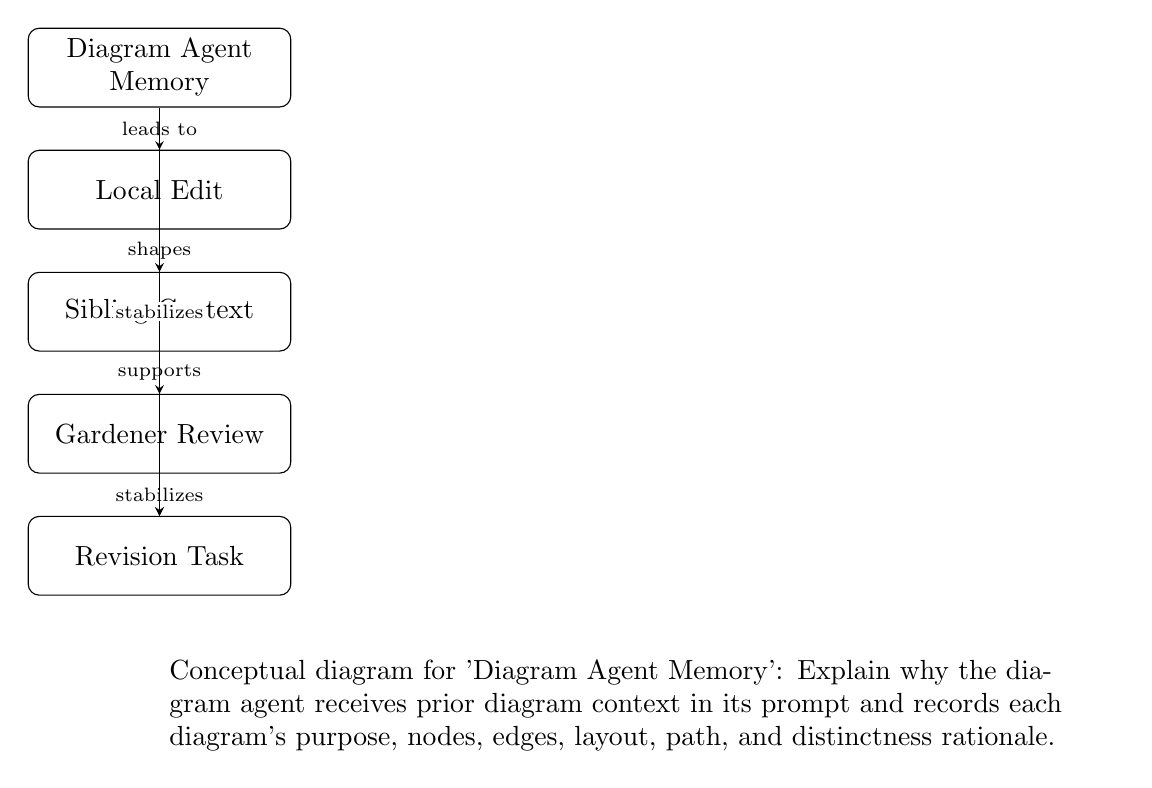
\begin{tikzpicture}[>=stealth, node distance=2.2cm,
  concept/.style={draw, rounded corners, align=center, text width=3.1cm, minimum height=1cm},
  relation/.style={font=\scriptsize, fill=white, inner sep=1pt}]
\node[concept] (n1) at (0,0.0) {Diagram Agent Memory};
\node[concept] (n2) at (0,-1.55) {Local Edit};
\node[concept] (n3) at (0,-3.1) {Sibling Context};
\node[concept] (n4) at (0,-4.65) {Gardener Review};
\node[concept] (n5) at (0,-6.2) {Revision Task};
\draw[->] (n1) -- node[relation] {leads to} (n2);
\draw[->] (n2) -- node[relation] {shapes} (n3);
\draw[->] (n3) -- node[relation] {supports} (n4);
\draw[->] (n4) -- node[relation] {stabilizes} (n5);
\draw[->] (n1) -- node[relation] {stabilizes} (n5);
\node[align=left, text width=12cm, anchor=north west] at (0,-7.4) {Conceptual diagram for 'Diagram Agent Memory': Explain why the diagram agent receives prior diagram context in its prompt and records each diagram's purpose, nodes, edges, layout, path, and distinctness rationale.};
\end{tikzpicture}

\caption{Conceptual diagram for ``Diagram Agent Memory'': explain why the diagram agent receives prior diagram context in its prompt and records each diagram's purpose, nodes, edges, layout, path, and distinctness rationale.}
\end{figure}


% CBM-SECTION-END:ch06_sec03_diagram_memory

\section{Drafting, Review, and Artifacts}

\subsection{Source Material and Section Payloads}

% CBM-SECTION-START:ch07_sec01_section_payloads:Source Material and Section Payloads

Imported source material for a section is the raw, pre-\LaTeX{} input that may arrive as markdown, outline notes, or other authoring fragments. It is useful as evidence of intent, but it is not yet the section payload that the compiler consumes. The section payload is the generated \LaTeX{} body for one specific section, written as a durable artifact in its own file and shaped to fit the surrounding manuscript.

This separation matters because the system treats source, transformation, and output as distinct state surfaces. Imported markdown can remain readable and editable as upstream material, while the section payload records the agent's current best rendering of that material in \LaTeX{}. Keeping those layers apart makes it possible to revise prose without overwriting the original source, to compare drafts against their inputs, and to inspect how a section changed over time.

Section agents therefore write only to section-specific \texttt{.tex} files such as \texttt{tex/section\_payloads/ch07\_sec01\_section\_payloads.tex}. That constraint keeps each agent's responsibility local: one agent owns one section payload, and no agent silently mutates the whole document. The result is easier review, clearer attribution, and fewer accidental cross-section edits. It also supports incremental compilation, because a changed section can be regenerated, diffed, and repaired without forcing unrelated sections to be rewritten.

In this workflow, the imported source remains the starting point, but the section payload is the artifact that downstream assembly uses. The payload is what enters proposal records, diffs, build logs, and compiled output. By writing only the section payload, the agent preserves a clean boundary between what was provided, what was inferred, and what is now ready for review.

This design is especially important in a multi-agent manuscript, where several agents may be drafting, revising, checking references, or responding to build feedback at the same time. A section-specific TeX file gives each agent a narrow, inspectable target and prevents the manuscript from becoming an opaque shared buffer. In short, imported markdown is source material; the section payload is the controlled \LaTeX{} realization of that source material; and the section file is the unit of ownership that keeps the system coherent.

That distinction also clarifies the artifact lifecycle described in this chapter. Source notes are not discarded when a section is rendered; they remain available as upstream evidence. The generated payload is the controlled output that can be reviewed, compared, and compiled. Later sections in this chapter extend that same logic to proposals, diffs, and repair loops: once a section exists as a separate payload, it can be tracked as a changeable artifact rather than as an invisible mutation of the manuscript.

Figure~\ref{fig:ch07_sec01_section_payloads} summarizes the distinction between imported source material and the section payload that section agents maintain.

\begin{figure}[htbp]
\centering
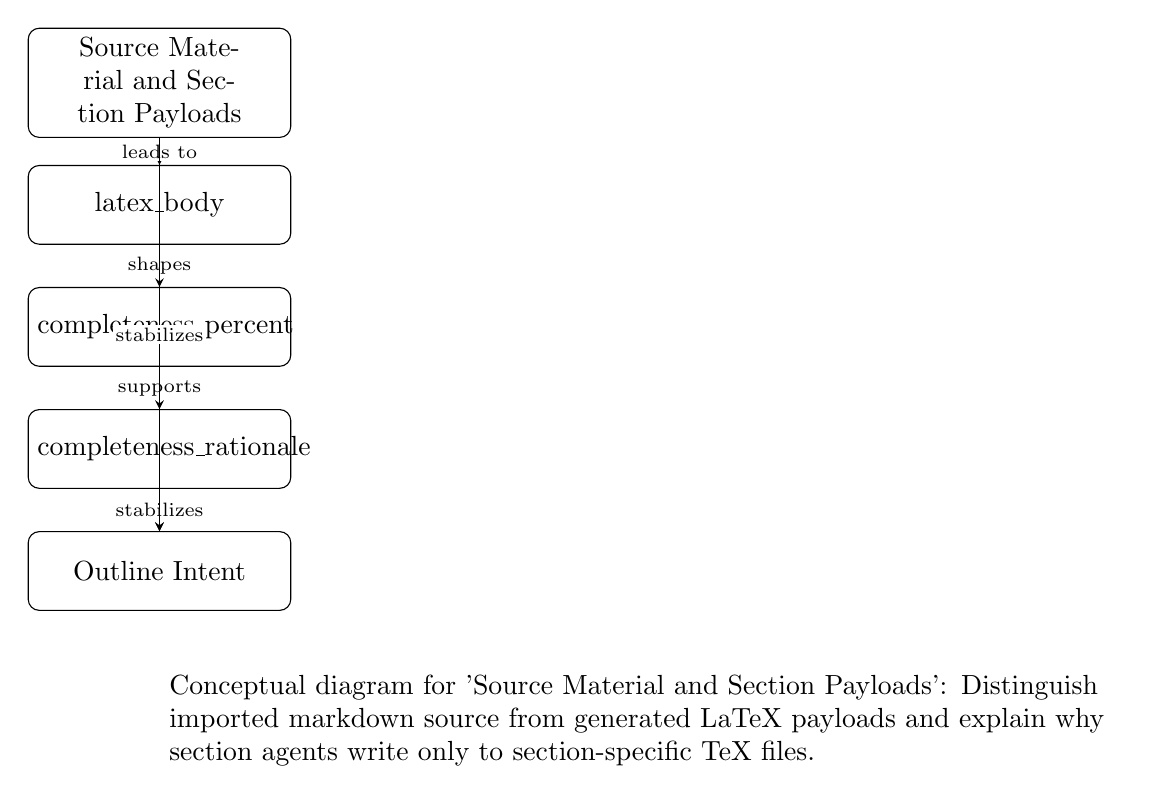
\begin{tikzpicture}[>=stealth, node distance=2.2cm,
  concept/.style={draw, rounded corners, align=center, text width=3.1cm, minimum height=1cm},
  relation/.style={font=\scriptsize, fill=white, inner sep=1pt}]
\node[concept] (n1) at (0,0.0) {Source Material and Section Payloads};
\node[concept] (n2) at (0,-1.55) {latex\_body};
\node[concept] (n3) at (0,-3.1) {completeness\_percent};
\node[concept] (n4) at (0,-4.65) {completeness\_rationale};
\node[concept] (n5) at (0,-6.2) {Outline Intent};
\draw[->] (n1) -- node[relation] {leads to} (n2);
\draw[->] (n2) -- node[relation] {shapes} (n3);
\draw[->] (n3) -- node[relation] {supports} (n4);
\draw[->] (n4) -- node[relation] {stabilizes} (n5);
\draw[->] (n1) -- node[relation] {stabilizes} (n5);
\node[align=left, text width=12cm, anchor=north west] at (0,-7.4) {Conceptual diagram for 'Source Material and Section Payloads': Distinguish imported markdown source from generated LaTeX payloads and explain why section agents write only to section-specific TeX files.};
\end{tikzpicture}

\caption{Conceptual diagram for ``Source Material and Section Payloads'': imported markdown source is distinct from the generated \LaTeX{} payload, and section agents write only to section-specific TeX files.}
\label{fig:ch07_sec01_section_payloads}
\end{figure}


% CBM-SECTION-END:ch07_sec01_section_payloads

\subsection{Proposals, Diffs, and Review}

% CBM-SECTION-START:ch07_sec02_proposals_and_diffs:Proposals, Diffs, and Review

In this system, an edit is not treated as an invisible mutation of the manuscript. It is first shaped into a proposal: a bounded change with an author, a target section, a rationale, and a traceable payload. That distinction matters because the book machine is designed to keep authorship legible at every step. A section agent does not silently overwrite text; it produces a section payload that can be inspected, compared, and revised before it becomes part of the durable manuscript state.

A proposal is therefore more than a draft. It is a reviewable unit of work that can carry metadata about where it came from, what task produced it, and which section it affects. In practice, this metadata lets the system distinguish a fresh draft from a later repair pass, a gardener-driven revision, or a callback triggered by another agent. The result is a manuscript history that can be reconstructed from durable records rather than inferred from the latest file contents alone. In other words, the proposal record preserves intent, the payload preserves the text, and the metadata preserves the circumstances under which that text was produced.

Diffs are the mechanism that makes those proposals legible. When a section changes, the system can compare the new payload against the prior version and expose the exact textual delta. That comparison is useful both for human review and for downstream automation. A reviewer can see what changed without rereading the entire section, and an agent can reason about whether the change is local, whether it introduces a new dependency, or whether it should trigger follow-up work in a sibling section. A diff is therefore not just a convenience for editors; it is part of the machine's coordination logic.

Checkpoints provide a second layer of durability. Instead of treating the latest text as the only state that matters, the machine can preserve intermediate versions as named or timestamped milestones. Those checkpoints make it possible to recover from a bad revision, to inspect the evolution of a section over time, and to separate experimental edits from committed ones. In a long-form technical document, that separation is especially valuable because a later repair may need to refer back to an earlier stable state rather than the most recent but still unverified draft. Checkpoints also make revision history easier to audit when a section has passed through several rounds of gardening or callback-driven repair.

This reviewable workflow also supports editorial accountability. A section agent can generate prose, but the prose remains provisional until it has passed through the system's review surfaces: the proposal record, the diff, and any subsequent repair or gardening pass. That means the manuscript is not a stream of opaque writes. It is a sequence of visible decisions, each of which can be attributed to a task, a message, or a callback in the runtime log. The point is not merely to keep a history; it is to keep a history that explains why the text changed.

The same principle applies to coordination between agents. If a gardener identifies a coherence issue, the resulting revision request is itself a durable artifact. If a reference is missing, the section agent does not fabricate support; it routes the need through the reference workflow and waits for a registered key before revising the text. If a diagram would materially improve the section, the request is explicit and the resulting asset is inserted only after the callback arrives. In each case, the system prefers a visible handoff over an implicit side effect. That preference keeps the manuscript's evolution inspectable even when several agents are working at once.

This is why proposals, diffs, and checkpoints belong together. Proposals define intent, diffs expose change, and checkpoints preserve recoverable states. Together they turn agent-authored editing into a reviewable process rather than a hidden mutation pipeline. That design keeps the manuscript inspectable, makes revision history durable, and gives both humans and agents a stable basis for further work. It also aligns this chapter with the surrounding sections: section payloads establish the owned text surface, while compilation and repair loops in the next section will show how those reviewable changes become buildable artifacts.

\begin{figure}[htbp]
\centering
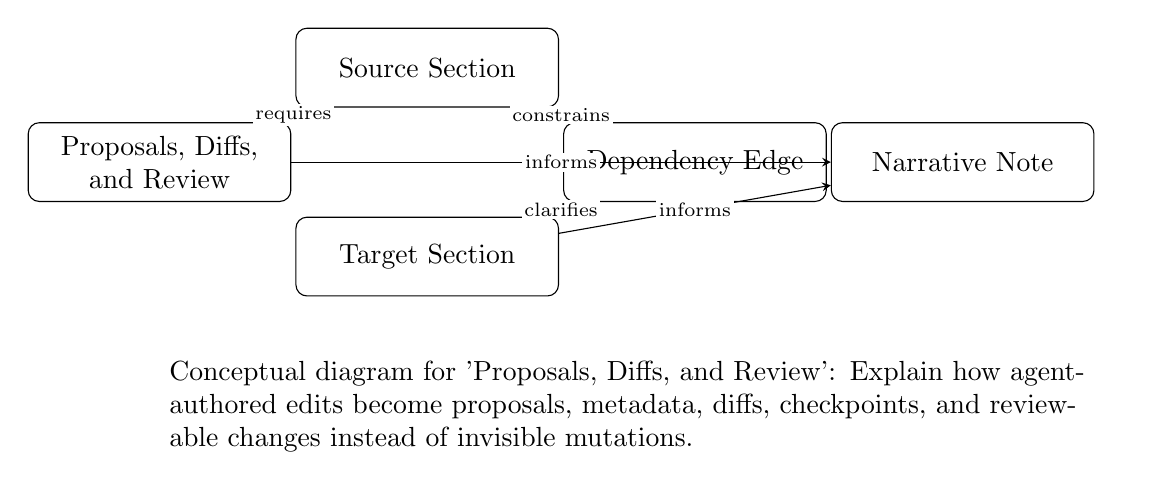
\begin{tikzpicture}[>=stealth, node distance=2.2cm,
  concept/.style={draw, rounded corners, align=center, text width=3.1cm, minimum height=1cm},
  relation/.style={font=\scriptsize, fill=white, inner sep=1pt}]
\node[concept] (n1) at (0,0) {Proposals, Diffs, and Review};
\node[concept] (n2) at (3.4,1.2) {Source Section};
\node[concept] (n3) at (6.8,0) {Dependency Edge};
\node[concept] (n4) at (3.4,-1.2) {Target Section};
\node[concept] (n5) at (10.2,0) {Narrative Note};
\draw[->] (n1) -- node[relation] {requires} (n2);
\draw[->] (n2) -- node[relation] {constrains} (n3);
\draw[->] (n3) -- node[relation] {clarifies} (n4);
\draw[->] (n4) -- node[relation] {informs} (n5);
\draw[->] (n1) -- node[relation] {informs} (n5);
\node[align=left, text width=12cm, anchor=north west] at (0,-2.4) {Conceptual diagram for 'Proposals, Diffs, and Review': Explain how agent-authored edits become proposals, metadata, diffs, checkpoints, and reviewable changes instead of invisible mutations.};
\end{tikzpicture}

\caption{Conceptual diagram for ``Proposals, Diffs, and Review'': agent-authored edits become proposals with metadata, are compared through diffs, and are preserved through checkpoints before they become reviewable manuscript changes.}
\end{figure}


% CBM-SECTION-END:ch07_sec02_proposals_and_diffs

\subsection{Compilation and Repair Loops}

% CBM-SECTION-START:ch07_sec03_compilation:Compilation and Repair Loops

This section closes the loop between generated prose and the compiled paper. Once section agents have written their payloads, the repository still needs a document-level assembly step that turns many isolated \texttt{.tex} fragments into a single buildable manuscript. In practice, that means the system must concatenate or \texttt{\input} the section payloads in outline order, resolve shared macros and package dependencies, and run the LaTeX toolchain against the assembled document until the build succeeds or produces actionable diagnostics.

The build log is not a disposable byproduct. It is a primary coordination surface for repair. A successful compile confirms that the manuscript is structurally consistent, while a failed compile identifies the exact file, line, and token context where the document broke. Because section payloads are owned by individual section agents, the repair loop should preserve that ownership boundary: the agent responsible for a section should receive the relevant diagnostics and make the smallest plausible correction to its own payload rather than rewriting unrelated material.

This minimal-repair discipline matters for two reasons. First, it keeps the provenance of changes legible: a compile error in one section should not trigger broad, speculative edits elsewhere in the book. Second, it reduces the risk of introducing new defects while fixing the old one. A section agent can usually respond to a diagnostic by correcting a missing brace, repairing an invalid citation command, adjusting an environment boundary, or rephrasing a sentence that overflows a fragile construct. The goal is not to optimize the prose in the same pass as the repair; the goal is to restore a clean build with the smallest safe change.

Compile diagnostics also support section attribution. When the assembler reports an error, the system can map the failing line back to the owning section payload and then to the corresponding section agent. That attribution is important in a multi-agent manuscript because the compiled document is a shared artifact, but the repair responsibility is local. The build log therefore functions as a routing mechanism: it tells the hypervisor or gardener which section agent should be asked to revise, and it gives that agent enough context to act without guessing.

Not every build issue is a syntax error. Some failures are editorial or design problems that only become visible after the manuscript is rendered. A page break may be awkward, a figure may be too large, a paragraph may create an undesirable widow or orphan, or a section may read correctly in isolation but feel unbalanced in the compiled layout. These are document-design feedback signals rather than pure compilation faults. They belong to the same repair loop, but they are routed differently: instead of asking for a mechanical fix to the TeX source, the system may ask for a local rewrite, a figure adjustment, or a layout-aware revision that improves the final page composition.

The important design choice is that compilation is not the end of authoring; it is a feedback stage. The manuscript is assembled, compiled, inspected, and then repaired in a bounded loop until the output is both syntactically valid and editorially acceptable. In that sense, the build log is part of the manuscript's memory. It records where the system failed, which section owned the failure, what kind of repair was needed, and whether the resulting document satisfied both LaTeX and design constraints. That durable feedback loop is what turns a collection of section drafts into a reliable compiled paper.

A practical repair loop therefore has three steps. First, assemble the manuscript from the current section payloads and run the compiler. Second, inspect the log and classify the failure as a local syntax problem, a missing dependency, or a document-design issue. Third, route the smallest appropriate task back to the owning section agent or to the document-level design workflow. This keeps the system from treating compilation as a monolithic pass and instead makes it a controlled exchange between build output and targeted revision.

In the broader chapter, this section completes the artifact lifecycle: source material becomes section payloads, section payloads become reviewable diffs, and reviewable diffs become compiled outputs that can still fail in ways worth repairing. The result is not merely a buildable manuscript, but a manuscript whose build history is itself inspectable and actionable.


% CBM-SECTION-END:ch07_sec03_compilation

\section{Implications and Open Questions}

\subsection{Design Principles}

% CBM-SECTION-START:ch08_sec01_design_principles:Design Principles

The Codynamic Book Machine is built around a small set of design principles that keep authoring work inspectable, recoverable, and easy to coordinate across agents. First, state is durable rather than ephemeral: outlines, section payloads, task queues, logs, and generated artifacts are written to repository-backed files so that the system can resume from recorded history instead of relying on hidden conversational memory. This makes the manuscript itself a persistent object, not a transient chat outcome.

Second, work is routed through explicit queues and visible messages. Agents do not silently mutate shared state; they receive declared tasks, choose an action that matches the task, and record their work as callbacks or append-only messages. That structure makes coordination legible to both humans and other agents, because each handoff can be inspected after the fact. It also reduces ambiguity about what was requested, what was completed, and what remains pending.

Third, the architecture assigns specialist ownership to distinct kinds of work. Section agents draft and revise section payloads, the gardener performs editorial maintenance, the references agent owns the shared bibliography, and the diagram agent manages visual assets and their memory. This division of labor keeps each agent focused on a narrow responsibility and prevents ad hoc edits from bypassing the system's checks. When a section needs support that it does not own, the request is routed to the appropriate specialist rather than improvised locally.

Fourth, edits are intended to be reversible and reviewable. Section payloads are stored separately from imported source material, so a draft can be regenerated, compared, or repaired without destroying the original notes. The same principle applies to revisions triggered by gardening or compilation feedback: the system prefers targeted changes over opaque rewrites, which makes it easier to understand why a line changed and to roll back if necessary.

Fifth, the system favors visible messages over hidden side effects. Inter-agent communication is represented as durable task records and readable chat lines, which means the coordination process itself becomes part of the manuscript's operational evidence. This visibility is important for debugging, editorial review, and later explanation of how a given section came to be.

Finally, the authoring workflow is schema-first. The canonical work object, its recursive outline, and the section payload model define the shape of the project before prose generation begins. By normalizing intent into structured fields and section-level responsibilities, the system can reason about dependencies, citations, diagrams, and compilation as parts of one coherent object. In practice, that means the prose is not merely written into a repository; it is authored within a machine-readable contract that keeps content, process, and artifacts aligned.

Taken together, these principles make the system less like a single-pass text generator and more like a durable editorial machine. The manuscript can be inspected at every layer, from outline to queue to \TeX{} to compiled artifact, while each agent remains accountable for a specific slice of the work. In that sense, the design principles are not abstract slogans; they are the operating rules that let the repository behave like a coordinated authoring system rather than a collection of loosely related files.


% CBM-SECTION-END:ch08_sec01_design_principles

\subsection{Limits and Failure Modes}

% CBM-SECTION-START:ch08_sec02_limits:Limits and Failure Modes

The system is most useful when it is disciplined about what it can and cannot do. Its strengths---durable state, explicit queues, specialist ownership, and visible messages---also define its failure modes. In practice, the same mechanisms that make the workflow inspectable can still produce repetitive prose, stale assumptions, over-eager visuals, or overconfident automation if they are not checked by editorial review.

One common failure mode is repeated generic output. When an agent is asked to draft a section from a short prompt, it may fall back on broad statements that sound plausible but do not add much local value. This is especially likely when the section topic is abstract or when the surrounding outline already contains similar language. The remedy is not to ask for more verbosity, but to require tighter alignment with the section's specific role in the outline, the surrounding sections, and the current state of the manuscript. A section draft should say something new about its own place in the system, not merely restate the paper's general thesis.

A related risk is stale memory. Because the workflow is distributed across task queues, callbacks, and separate section payloads, an agent can easily reason from an outdated view of the manuscript. A section may continue to reflect an earlier outline, an older dependency, or a superseded editorial decision. Durable logs help expose this drift, but they do not eliminate it. The practical safeguard is to re-read the current outline, sibling sections, and registered references before revising, and to treat any callback or gardener note as a signal that the local context may have changed.

Diagrams introduce another class of failure. Visuals are useful when they clarify a workflow, but they can become over-eager when every concept is forced into a figure. A diagram request should be justified by a concrete explanatory gain: a queue lifecycle, a handoff pattern, or a dependency structure that is easier to understand visually than in prose. Otherwise, the manuscript risks accumulating decorative figures that repeat the text instead of sharpening it. The diagram workflow therefore needs restraint as well as capability.

Unsupported claims are a more serious problem. The system can describe its own behavior from logs and repository state, but it should not present conjecture as fact. If a section needs a claim about implementation details, performance, or external practice that is not already grounded in the repository, it should either be supported by a registered reference or rewritten as a bounded observation about the current system. This is especially important in a paper that presents a working system as evidence: the prose should distinguish what is observed in the repository from what is inferred or proposed.

Prompt and context size also impose hard limits. A section agent can only reason over a finite slice of the manuscript, and long outlines, large logs, or extensive sibling context can crowd out details. This means the system must rely on decomposition: section-level ownership, explicit dependencies, and targeted revision tasks. Even so, some global coherence problems will not be visible from a single section pass. The architecture reduces context pressure, but it does not abolish it.

For that reason, human review remains necessary. The machine can draft, compare, route, and repair, but it cannot fully arbitrate style, emphasis, or the final balance between precision and readability. Human oversight is the last defense against subtle repetition, misplaced confidence, and architectural blind spots. In this sense, the system is not a substitute for editorial judgment; it is a way to make that judgment more informed, more traceable, and easier to apply at scale.

The limits of the Codynamic Book Machine are therefore not incidental. They are the predictable edge cases of a system that makes its own work visible. By exposing repetition, drift, unsupported claims, over-eager diagrams, and overreach as explicit failure modes, the architecture gives the author and editor a clearer basis for intervention. That visibility is the point: the machine is designed not to eliminate judgment, but to make judgment easier to exercise well.


% CBM-SECTION-END:ch08_sec02_limits

\subsection{Future Work}

% CBM-SECTION-START:ch08_sec03_future_work:Future Work

This section identifies the most promising directions for extending the Codynamic Book Machine beyond the current implementation. The present system already demonstrates durable work objects, explicit task queues, specialist agents, and a reviewable artifact pipeline, but several capabilities remain intentionally underdeveloped. The most immediate opportunities are to make diagram planning more semantically aware, to improve how revision work is scheduled across the whole manuscript, to strengthen retrieval and registration of references, to expose more of the runtime state in the user interface, and to evaluate the system more formally against repeatable criteria.

First, diagram support could move from opportunistic requests toward richer planning. At present, section agents can propose one or two diagrams when a visual would materially clarify a section, but the decision is local and largely manual. A more capable planner could inspect the outline, the dependency graph, and prior diagram memory to identify recurring structures that deserve consistent visualization across chapters. For example, the system could distinguish between architecture diagrams, workflow diagrams, and state-transition diagrams, and it could avoid redundant figures by comparing proposed diagrams against previously generated assets. Such a planner would make diagram generation less reactive and more aligned with the manuscript's conceptual structure.

Second, revision scheduling could become more global and less purely section-local. The current gardening cycle is effective at catching local drift, repeated claims, and unsupported assertions, but it still depends on targeted callbacks and incremental maintenance. A future scheduler could rank revision work across the entire book by severity, dependency depth, and downstream impact, then batch related edits so that cross-references, terminology, and narrative transitions are repaired together. This would be especially useful when a change in one chapter affects definitions or phrasing in later chapters. A global scheduler could also reduce churn by preventing multiple agents from revising the same conceptual area in isolation.

Third, reference retrieval and registration could be made more robust. The present workflow correctly separates citation ownership from section drafting, but it still relies on the agent to notice missing support and to request research at the right time. Future work could add stronger claim-to-source matching, better detection of unsupported technical statements, and more structured handoff records for references\_agent. In addition, the system could surface citation gaps earlier in the drafting process, before prose is finalized, so that unsupported claims are less likely to survive into later review stages. This would improve both factual reliability and the efficiency of the editorial loop.

Fourth, the user interface could expose more of the system's internal state without overwhelming the reader. Because the machine is built around durable queues, append-only messages, and generated artifacts, it is well suited to observability. A richer UI could show task status, pending callbacks, revision history, diagram requests, citation registration state, and build outcomes in a single place. It could also make it easier to inspect why a section changed, which agent made the change, and what evidence or feedback triggered the revision. Better observability would not only help operators debug the system; it would also make the architecture easier to trust and explain.

Finally, the system would benefit from more formal evaluation. The current paper is grounded in a working repository, but the evidence is still primarily qualitative and case-study based. Future work could define benchmarks for revision quality, citation completeness, diagram usefulness, build stability, and turnaround time across repeated editing cycles. It could also compare the Codynamic Book Machine against simpler pipelines that lack durable queues or specialist agents. Such evaluation would help distinguish which parts of the architecture are essential, which are merely convenient, and which produce measurable gains in long-form authoring.

Taken together, these directions point toward a more autonomous, more legible, and more empirically grounded book machine. The current system already shows that books can be treated as coordinated technical artifacts; future work is about making that coordination deeper, more observable, and easier to validate.


% CBM-SECTION-END:ch08_sec03_future_work

\end{document}
